\documentclass[../../main.tex]{subfiles}

% Image numbers: 10-201 inclusive

\begin{document}

\newchapter{Design Process}{design-process}

\section{Preliminary design} \label{sec:design-process:preliminary-design}

\subsection{Operation and initial constraint analysis} \label{sec:design-process:preliminary-design:operation-and-initial-constraint-analysis}

To size the propulsion systems, initial analysis was conducted by estimating a number of design and environment parameters, using a normal distribution around each one to form a distribution of the most likely power requirement.
From this, early estimates of crucial parameters such as motor power, wingspan, and aspect ratio could be made.

The cruise speed was estimated using preliminary values of mass, \cl, aspect ratio, and span.
The function is shown in Appendix \ref{appendix:calculation-process-for-initial-parameter-selection}.
This function could then be used to form a probability distribution, shown in Figure \ref{fig:cruise-distribution:velocity}, and hence the most likely value of the cruise velocity based on the estimated values.
It was found that the mean and median both have values of approximately \mps{21}, and so this was taken as the estimated cruise velocity during the initial phases of the project. 

The power requirements could then be estimated using a similar procedure, taking preliminary values for efficiency, mass, \vcruise \, (as estimated above), \cl, and \cd, again using normal distributions of unknown values (Appendix \ref{appendix:calculation-process-for-initial-parameter-selection}).
This was then be used to find the probability distribution for the power required in cruise, shown in Figure \ref{fig:cruise-distribution:power}.

\begin{figure}[H]
    \centering
    \begin{subfigure}[b]{0.49\columnwidth}
        \centering
        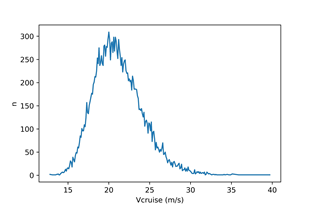
\includegraphics[width=\textwidth]{cruise-velocity-distribution}
        \caption{Velocity}
        \label{fig:cruise-distribution:velocity}
    \end{subfigure}
    \hfill
    \begin{subfigure}[b]{0.49\columnwidth}
        \centering
        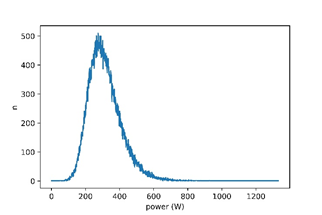
\includegraphics[width=\textwidth]{cruise-power-distribution}
        \caption{Power}
        \label{fig:cruise-distribution:power}
    \end{subfigure}

    \caption{expected distribution of selected properties during cruise.}
    \label{fig:cruise-distribution}
\end{figure}

The mean value of the power required in cruise was found to be \watts{315}, with a median of \watts{302}, giving an estimated power requirement in cruise of around \watts{310}.
There is more uncertainty in power than \vcruise\, due to the larger range of values covered within one standard deviation of the mean, but this still provided a good starting point for the project.

\subsection{Further constraint analysis} \label{sec:design-process:preliminary-design:further-constraint-analysis}

Using the refined parameters found in \S \ref{sec:design-process:preliminary-design:operation-and-initial-constraint-analysis}, design decisions made, and further analysis of the UAV, the constraint analyses were combined to show all parts of the flight profile and hence find the minimum power requirement.
This code gave more refined estimates for the power requirement in different areas of the flight envelope, as well as takeoff speed, which could be updated quickly and easily as design decisions were made and various operational parameters were refined.
Figure \ref{fig:constraint-analysis} shows the final plots after all research and design decisions were made.

% \importimage{full-constraint-analysis}{full constraint analysis plot with feasible region highlighted.}{Full constraint analysis}{0.85}
% \importimage{takeoff-speed-plot}{takeoff speed plot.}{Takeoff speed plot}{0.85}

\begin{figure}[H]
    \centering
    \begin{subfigure}[b]{0.85\columnwidth}
        \centering
        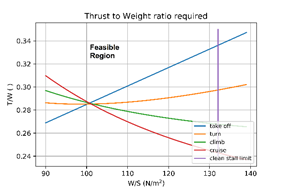
\includegraphics[width=\textwidth]{full-constraint-analysis}
        \caption{Feasible region}
        \label{fig:constraint-analysis:full}
    \end{subfigure}
    \hfill
    \begin{subfigure}[b]{0.85\columnwidth}
        \centering
        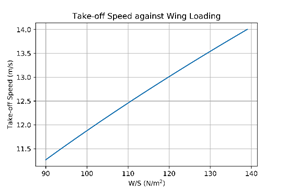
\includegraphics[width=\textwidth]{takeoff-speed-plot}
        \caption{Takeoff speed}
        \label{fig:constraint-analysis:takeoff-speed}
    \end{subfigure}

    \caption{full constraint analysis plot with the feasible region highlighted.}
    \label{fig:constraint-analysis}
\end{figure}

It can be seen that the lowest thrust to weight ratio required is around 0.29, which corresponds to a power requirement of around \watts{520}; though this is for a wing loading of only \npmsq{100}.
The final wing loading of ELMO UAV turned out to be approximately \npmsq{111}, giving a thrust to weight requirement of just over 0.3 and a corresponding power requirement of around \watts{650}, and so the final selection of motors was sufficient with a small amount of power to spare. 

\subsection{Wing} \label{sec:design-process:preliminary-design:wing}

Early in the project due to its nature, the complexity of certain components, and the limited budget, it was decided that a simple rectangular wing would be used on the UAV.
Taking the modularity onto account, a rectangular wing would reduce the number of engine housing units needed, therefore reducing the amount of design and manufacturing, and hence the cost of the project. 

The UAV had a \metres{2} span, with a fixed chord of \cm{30}, which gave an aspect ratio of 6.6.
The chord length was initially at \cm{25}, closer to the desired aspect ratio of 8.
Concerns regarding the size of flaps and ailerons were raised, however, as a significant amount of the wingspan would be lost to the motor housing units, so the chord length was increased to \cm{30} as a compromise.  

Once a wing shape had been decided, a more detailed analysis of possible aerofoil sections took place.
Initial 2D simulations were run on XFLR \cite{xflr-19} to narrow the choice down to five aerofoils.
The analysis was run at a Reynolds number of \stdf{1.35}{6}, calculated using standard atmospheric conditions at a cruise speed of \mps{20} and a reference length on XFLR of \metres{1}. 

Although the purpose of the project was to improve the efficiency of electric aircraft by altering the position of the propulsion units, the aim was not to produce the most efficient aircraft; moreso a test craft which can be reused to run experiments at a lower cost than a wind tunnel.
Therefore, when choosing the aerofoil, the main considerations where not only $L/D$ but also stall angle, maximum \cl, and moment coefficient, amongst others.
The analysis narrowed down to four potential aerofoils: the Clark Y, S1223, NACA6412, RG15A213, whose coordinates were taken from Airfoil Tools \cite{airfoil-tools-19}.
Figure \ref{fig:alpha-characteristics} shows the \cl, \cl$/$\cd, and \cm\, curves respectively for four suitable aerofoils. 

The Clark Y (blue line) is very common among model UAV makers because of its gentle stall angle at around \degr{12}, with a further sharper drop off at around \degr{20}.
It also has a gentle moment coefficient which makes it stable to changes in attitude during flight. 

The S1223 (black line) has an extremely high $L/D$ ratio due to its high camber; it also has a slightly higher stall angle than the Clark Y (at around \degr{14}).
It has an unfavourably large moment coefficient, however, which may make it unstable in flight.
Its high camber and narrow trailing edge may also make it difficult to implement high lift devices, as well as it not being strong enough to support a tractor propulsion set up.

The NACA6412  (green line) has a high $L/D$ ratio up to \degr{10} of incidence as well as a higher \cla\, curve, which is useful as a large part of the wing wetted area will be taken by motor housing.
It has a slightly higher moment coefficient than the Clark Y at low angle, though, as well a lower, yet gentle, stall angle of \degr{11}.

The RG15A213 (red line) has the lowest \cla\, of the five, but has a higher stall angle at \degr{15} as well as having the lowest moment coefficient.

Of the five aerofoils above, further analysis would be carried out on the Clark Y and the NACA6412 aerofoils as they provided good lift performance, strong lift to drag ratio, and a manageable moment coefficient.

\importimage{alpha-characteristics}{variation of \cl, \cl$/$\cd, and \cM\, with $\alpha$.}{Angle of attack characteristics}{0.9}

\subsection{Fuselage} \label{sec:design-process:preliminary-design:fuselage}

Given the project objectives, the design of the UAV was based around commercial aircraft, discounting any lightweight or double fuselage seen on many UAVs such as SPOTTER \cite{spotter-19}. 
Initial designs included a square, circular, and aerofoil-shaped fuselage.

\importtable{| >{\raggedright\arraybackslash}p{0.12\columnwidth} | >{\raggedright\arraybackslash}p{0.36\columnwidth} | >{\raggedright\arraybackslash}p{0.36\columnwidth} |}{
    \hline
    \textbf{Design} & \textbf{Advantages} & \textbf{Disadvantages} \\
    \hline
    Square & Easy manufacturing and wing attachment; strong structural performance & Poor aerodynamics \\
    \hline
    Circular & Easy to manufacture & Hard to attach wing; difficult to create internal structure \\
    \hline
    Aerofoil & Aerodynamic; aesthetically pleasing & Difficult to manufacture \\
    \hline
}{tradeoffs involved in the type of fuselage design.}{fuselage-tradeoffs}

\importimage{potential-aerofoil-design}{potential aerofoil fuselage design.}{Potential aerofoil design}{0.5}

For the wind tunnel model, it was decided that a hybrid of a square fuselage and an aerofoil shaped fuselage would be beneficial.
It was thought that a side profile of a NACA0012 aerofoil would reduce drag and increase lift, whilst a square front section would make manufacturing easier.
This would give a combination of aerodynamic design and ease of manufacturing.  
The NACA0012 was chosen as a suitable aerofoil as it would provide enough height to hold all of the electronics, as well as enough room to reach inside if needed. 
The initial fuselage design was \metres{1.5} long, with a width of \mm{175} and a height (at the thickest part) equal to around \mm{180}. 

\subsection{Tail} \label{sec:design-process:preliminary-design:tail}

Note that for many of the tail and control surface mathematical design processes, details of the equations used are unnecessary for understanding; but for the interested reader can been found in the appendices. 

The tail was designed with a volume coefficient process.
First, volume coefficients were estimated from Table 9.4 in Raymer \cite{raymer-89}, and a value of 0.8 was selected for the horizontal and 0.07 for the vertical tail volume.
Next, values for tail surface aspect ratios were estimated as 5 for the horizontal tail, and 2 for the vertical tail from Table 9.1 in Raymer.
The formulae for vertical and horizontal tail volume coefficients for tailplane areas were rearranged to obtain the vertical and horizontal tail areas, where the aspect ratio selected could then be used to determine span, and then MAC of the tail surfaces.
Lastly, the taper ratio was used to determine root and tip chords of the tail surfaces.
At this stage, no setting angle was determined as the need for this had not yet been recognised. 

Next, the spars had to be sized for the wind tunnel test.
Upon advice, they were sized for $10g$ loads \cite{towell-19}.
A simple mathematical beam model was used to size the spars in the tail as well as the main structural arm.
The horizontal tail spars were modelled as having a $5g$ (\newtons{49.05}) load distributed evenly over the semi-span.
Based on values for the inner and outer diameters of the spars, length, and chosen material stiffness, the tip deflection was found.
The main structural arm was determined by modelling a $10g$ point load in line with the horizontal spars, and using inner and outer widths instead of diameters, as it was decided that this would be a square section to prevent parts rotating around it.

\subsection{Control surfaces, electronics, and avionics} \label{sec:design-process:preliminary-design:control-surfaces-electronics-and-avionics}

The initial design was with the first wind tunnel test in mind, and as such had no plans for functional control surfaces, electronics, or avionics.
It was hoped that the first test would finalise the basics of the fuselage, wing, and tail geometry, and highlight where changes would be required from the initial design
Subsequent models and tests could validate the performance of more complex aspects of the UAV. 

Work did begin, however, on selecting and configuring a flight controller.
The primary role of the flight controller is to convert control inputs from the pilot into control inputs that are sent directly to the servos, and is normally accomplished through a range of techniques, including PID controllers.
Two main flight controllers were investigated, the first being a Pixhawk flight controller $-$ more expensive, but potentially more useful and had been used by people at the university before $-$ and the second being a Matek F405-Wing board with iNav Flight firmware installed on it. 

While the Pixhawk could have been easier to set up, with its advertised plug-and-play functionality, it was significantly more expensive, and so it was decided that looking into the Matek controller could be worth a potentially large saving (albeit with a greater risk of purchasing the controller to find that it did not work as expected).
The Matek hardware came at about half the cost of the Pixhawk, and while the corresponding firmware was relatively immature, its open source nature meant that its functionality was expanding quickly, and it had favourable reviews from a number of online sources.
Another potential advantage of the Matek controller was that it was designed specifically with fixed wing aircraft in mind, whereas the Pixhawk was focused more towards quadcopters. 

\importimage{matek}{pin layout and documentation for the Matek flight controller.}{Flight controller layout}{0.95}  % TODO: include source (http://www.mateksys.com/?portfolio=f405-wing)

Other beneficial features of the Matek board were the built-in current sensor and inertial measurement unit (IMU) which would provide estimates of the position, and more importantly orientation, of the UAV.
There were also a number of fairly low-cost GPS and airspeed sensor units, required for the latter part of the avionics system's specification of providing autopilot functionality. 

\importimage{flight-configurator}{flight configurator software used to set up the flight controller.}{Flight configurator}{0.6}

Input to the flight controller could be achieved through a number of protocols, most notably through SBUS; this type of serial connection appeared to be the most commonly supported amongst receivers, and would allow up to sixteen channels to be passed from the receiver to the controller.
The minimum required channels would be eight: four for throttle, yaw, pitch, and roll; two for flaps (on/off); and similarly two for the autopilot toggle.
With the additional channels it would in principle be feasible to implement extra features, such as manually cutting off outboard motors in the event that one of them should fail. 

Also of interest were the UART ports (Figure \ref{fig:matek}), which is a serial communication protocol broadly compatible with a number of microcontrollers, including Arduinos.
This would be a good option for extracting the data from the current sensor and passing it to a microcontroller $-$ most likely an Arduino Nano $-$ which could then integrate the current draw over time to provide an estimate of the battery capacity used by a particular configuration.
Being able to do this onboard was appealing because the need for telemetry, which would have significantly increased the complexity of the radio system, could be removed.
All data could be logged by a relatively simple program, written in C++, to be downloaded after each flight. 

\importimage{flight-controller-computer}{flight controller plugged into a computer running the flight configurator.}{Flight controller configuration}{0.6}
\importimage{flight-controller-receiver}{receiver undergoing the binding procedure.}{Receiver binding}{0.5}

\subsection{Propulsion} \label{sec:design-process:preliminary-design:propulsion}

\subsubsection{Twist-in motor attachment} \label{sec:design-process:preliminary-design:propulsion:twist-in-motor-attachment}

\begin{figure}[H]
    \centering
    \begin{subfigure}[b]{0.49\columnwidth}
        \centering
        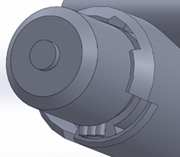
\includegraphics[width=\textwidth]{twist-in-in-place}
        \caption{Motor in-place in housing}
        \label{fig:twist-in:in-place}
    \end{subfigure}
    \hfill
    \begin{subfigure}[b]{0.49\columnwidth}
        \centering
        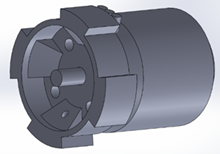
\includegraphics[width=\textwidth]{twist-in-attached}
        \caption{Bracket attached to motor}
        \label{fig:twist-in:attached}
    \end{subfigure}

    \begin{subfigure}[b]{0.49\columnwidth}
        \centering
        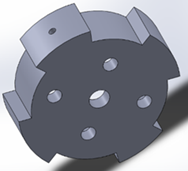
\includegraphics[width=\textwidth]{twist-in-bracket}
        \caption{Bracket}
        \label{fig:twist-in:bracket}
    \end{subfigure}
    \hfill
    \begin{subfigure}[b]{0.49\columnwidth}
        \centering
        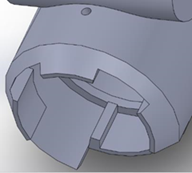
\includegraphics[width=\textwidth]{twist-in-housing}
        \caption{Housing}
        \label{fig:twist-in:housing}
    \end{subfigure}
    \caption{CAD models of the twist-in motor attachment used in the tail.}
    \label{fig:twist-in}
\end{figure}

Conceived early in the project's development, the twist-in motor attachment (Figure \ref{fig:twist-in}) was a proposed design for the attachment of the wing motors.
When the design criteria changed to include a battery and ESC in the movable propulsion unit, a new design was required.
This design, however was still used in the tail section as the battery and ESC were fixed in the fuselage for that configuration, and so only the motor moves, making this an ideal solution.

The design is intended to allow for quick and simple removal and replacement of the motor when changing configurations of the UAV in order to reduce ground time at the flying days.
This utilises a twist and fix design where four tabs on the bracket, shown in Figure \ref{fig:twist-in:bracket}, which attaches to the back of the motor as shown in Figure \ref{fig:twist-in:attached}, engage with four tabs in the housing, and the motor then rotates up to a limiting piece to align the bracket and housing (Figures \ref{fig:twist-in:housing} and \ref{fig:twist-in:in-place}).
The motor is then secured in place using a small grub screw which engages with the bracket through a clearance hole in the top of the housing, as shown in Figure \ref{fig:twist-in:housing}, providing resistance to rotation of the motor while the tabs provide the strength in the direction of the force of the motor.
The large cut-out in the housing is to allow room for the wires of the motor when it is being fitted, as they protrude from the rear part of the motor out to the side, shown in Figure \ref{fig:twist-in:in-place}.
On the final design for the tail there is a full routing designed for the wires but that was not designed here as this housing was intended for the wing before being deprecated.

\subsubsection{Sizing} \label{sec:design-process:preliminary-design:propulsion:sizing}

Initial sizing started from the constraint analysis' power requirement estimations, allowing motors to be selected.
The constraint analysis at this point suggested a power requirement of around \watts{600}, and so motors of around this power were researched from a recommended supplier Outlander, and a number of suitable cost-effective motors were found for both the fuselage and wing locations, as listed in Figure \ref{fig:unknown}.  % TODO: find needed figure
These were then used to find suitable ESCs, which were recommended for the motors as \amps{60} and \amps{30}, but due to this being the most common part to fail on previous projects due to overloading, a decision was made to oversize the ESCs by \pc{30} and so \amps{40} and \amps{80} ESCs were selected.
The batteries were then chosen based on the voltage and current requirements of the motors, meaning that they needed to be 4S to provide the required \volts{14.8}, and the capacity initially chosen simply on weight and cost, with the largest capacity shown being the heaviest that could be used.
The C value is used to find the maximum current output of the battery and so this was chosen to ensure a large safety margin between the maximum of the battery and the maximum of the motor, reducing any chance of the battery overheating while in use. 

The motor selection was then refined due to an increase in the power requirement prediction from the constraint analysis resulting from updates to the UAV design; this meant that the motors could be selected as the Tornado Thumper V3 3548/05 and 3530/14 for the fuselage and wing motors respectively.
This meant that the battery capacities could be checked for time of flight based on an estimated \pc{75} throttle average throughout a flight.
While this is an overestimate, it gives a useful conservative estimation of the flight time.
This showed that the smaller capacity batteries would not be enough to provide a flight time suitable for recording the needed data while having a margin in the battery to avoid a power cut-out mid-flight.

Along with finalising the battery selection, the propellers could now be researched as shown in Figure \ref{fig:unknown}.
This initially required the maximum propeller diameter to be found for the motors, based on the max RPM of the motor, which would give a Mach number of the propeller of around 0.7, which would maximise thrust without having large increases in power requirement due to transonic effects at the blade tip.
This was then used to refine an iterative search of the available propellers from APC, a manufacturer trusted by the university.
The advance ratio was found based on the blade diameter, RPM, and a target maximum flight speed of \mps{25}, and then a suitable propeller was found in the database that had a power draw similar to that of the maximum of the motor at the target flight speed and RPM, while providing enough thrust based on estimations of the aircraft drag.

These propellers were checked after selection at the target cruise speed of \mps{20} to ensure that the thrust would be adequate, and to find an estimation of the efficiency in order to further refine the constraint analysis.
The ideal propellers, however, could not be used due to the specific use case of the project, which requires both tractor and pusher configurations to be employed, as well as counter rotating propellers on each wing; this meant that the propeller would need to have an equivalent pusher propeller.
The selection of propellers was therefore forced into suboptimal blades, with the fuselage propeller only having one viable option of the APC 12x6E and 12x6EP propellers, and the wing having two options of the 8x6E and 7x5E.
After analysis of thrust data, the 8x6E was chosen to be used in a motor and propeller wind tunnel test to verify that this propeller would be suitable, and to verify the quoted performance data in order to ensure that the 12x6E would also be suitable. 

\section{Physical testing and validation} \label{sec:design-process:physical-testing-and-validation}

\subsection{Wind tunnel test} \label{sec:design-process:interim-design-review:wind-tunnel-test}

\subsubsection{Fuselage} \label{sec:design-process:interim-design-review:wind-tunnel-test:fuselage}

The fuselage was designed around a hollow \metres{1} long and \mm{20} square aluminium boom as its core structural element.
Around the boom was a foam and poplar plywood structure, similar to the wing. 

The driving force behind the fuselage design was the need to be able to change the setting angle of the wing with ease.
As a result, the metal boom was fixed to four layers of poplar ply ribs which ran the length of the fuselage. 

To allow the wing setting angle to be changed easily, three sets of holes ran through the fuselage.
The front set of holes were a tight fit for the front spar, so it could not move.
The middle set was a guide for the rear spar to help changing the angle.
The rear set of holes were to secure the wing in place.
This section contained seven holes in total, each \degr{2} apart, meaning the wing's angle could be changed from \degr{0} up to \degr{12}. 

\importimage{fuselage-cross-section}{a cross-section of the fuselage, showing the structure and hole layouts.}{Fuselage cross-section}{0.6}

At the rear of the model, on the underside, the middle two ribs contained an attachment point for the wind tunnel.
This was extruded from the model to enable the model to be easily attached and removed from the struts. 

\importimage{laser-cut-plywood}{laser-cut plywood for the fuselage.}{Laser-cut plywood}{0.7}

\subsubsection{Wing} \label{sec:design-process:interim-design-review:wind-tunnel-test:wing}

The wing was constructed using two hollow aluminium spars as the key structural elements with the front spar at quarter chord and the rear spar at half chord, with outer diameters of \mm{15.88} and \mm{12.7}, respectively.
Each spar was \metres{2} long and ran tip to tip through the fuselage.
Surrounding the spars was blue styrofoam, cut in the university's foam cutter.
Separating the foam sections were \mm{3} thick poplar ply ribs, cut on university's laser cutter.
Each rib had a unique design and were individually designed and cut.

\importimage{flap-dfx-file}{DFX file of flap rib for the Clark Y aerofoil section, later used for laser cutting.}{Flap DFX file}{0.6}

There were six ribs used in each wing half, in locations that would roughly replicate where the motor housing units would be on the final model.
Therefore, the ribs were located either side of the flap and \mm{130} outboard.
The next rib, located \mm{101} outboard, was the rib used to connect the model to the wind tunnel.
Therefore, it was made from \mm{6} birch ply as this provided sufficient strength for an integral component.
The two final ribs were located at the wing tip and \mm{50} inboard.

\importimage{underside-of-wing}{the underside of the wing, showing attachment and flap adjustment methods.}{Underside of wing}{0.6}

The thicker birch ply rib, located \mm{700} outboard of the centre of the aircraft, contained an extrusion with a hole for an M6 bolt to allow easy attachment and removal to the wind tunnel mounts.
Its location along the wing was dictated by the wind tunnel mounts. 

The foam and ribs for each side of each wing were bonded together using epoxy resin but were not bonded to the spars themselves, allowing the wing sections to be removed from the spars during the wind tunnel test. 
The wings were secured to the wing using two 3D printed clamps on each spar. 

\importimage{internal-spar-structure}{Wing section showing the internal spar structure.}{Internal spar structure}{0.6}

\subsubsection{Control surfaces} \label{sec:design-process:interim-design-review:wind-tunnel-test:control-surfaces}

The main purpose of the wind tunnel model was to cement top level parameters such as aerofoil section, setting angle, chord length, and wingspan.
As a result, the wind tunnel was unpowered, and ailerons were not included in the model.
It was, however, important to test the effect of a flap on each wing and which aerofoil would be more amenable to the addition of a flap. 

Initial research suggested that, for a typical low-speed UAV, ailerons take up approximately \pc{40} of the semi-span, in this case \mm{400} \cite{sadraey-13}.
This left the remaining \pc{60} for flaps.
The design at the time, however, called for the motor housing units to have width of approximately \mm{110}.
There would be two located on each half of the wing, and a tip mounted motor, whose depth had not yet been determined.
The flaps were therefore set to a width of \mm{380}, which would act as a worst case scenario approach to the design, and would provide each wing section with a strong test.

The flaps were designed to be changed manually whilst the model was still attached to the wind tunnel.
The guides either side of the flaps had M2 holes every \degr{5} up to \degr{35}.
As the flap angle was altered, two M2 bolts would secure the flap in place. 

\importimage{flap-mechanism}{close up of the flap mechanism.}{Flap mechanism}{0.6}

\subsubsection{Tail} \label{sec:design-process:interim-design-review:wind-tunnel-test:tail}

With the mathematical modelling complete, a 3D model of the tail surfaces could be created as reference for building.
This was done by defining the sketch planes upon which the roots and tip chord aerodynamic profiles would be created, importing curves of the aerofoil from coordinate files, and parametrising them (by chord length and angle of attack) so that they could be manipulated.
Lofted bases were created between the profiles, then additional details such as cut-outs for spars were added.
This was repeated for all three control surfaces, and then simple models of the tail spars and main structural arm were created and added to the overall assembly. 
The initial plan was to use the foam cutter to create the tail profiles, however, this proved to be infeasible as the cut-outs for the spars in a thin aerofoil profile (NACA0012) left very little foam in the wall which resulted in the foam melting at the tip where the cutter had to slow down.  

There was not enough time to redesign the tail because of the upcoming test, so it was decided to laser cut wooden profiles at equally spaced intervals along the tail surfaces and wrap Solarfilm around them.
Geometry was created in CAD using repeated \mm{3} profiles intersecting the foam geometry, and then non-intersecting geometry was deleted to leave the laser cut profiles, which were quickly exported and cut.
Each profile was mounted and bonded to the spar.
Once the glue had cured, Solarfilm was wrapped around the profiles, with the leading and trailing edges stiffened with card.
While this was messy, it was effective; it was resolved to refine the model for the next iteration of the design.  

The tail was mounted on the model using a friction fit with the spars running through the fuselage and main structural arm.
Holes were drilled through these that were intentionally half a millimetre short of the spacing required.
One horizontal tail surface was glued to one spar, and the other to the second, so they would slot together neatly in the model.
The vertical tail surface contained both spars, and simply slotted in all at once. 

\importimage{wind-tunnel-model}{final wind tunnel model.}{Wind tunnel model}{0.8}

\subsubsection{Test plan} \label{sec:design-process:interim-design-review:wind-tunnel-test:test-plan}

The wind tunnel test had a few objectives.
The first was to validate the designs produced so far, ensuring that lifting surfaces could produce sufficient lift and were able to withstand the predicted structural loads.
Assuming these conditions were met, a combination of aerofoil, wing-body angle, and flap-wing angle needed to be found which optimised the objective function (discussed later in more detail).
Data collected during this optimisation would also be used afterwards to refine the design further $-$ by estimating the change to lift or drag that would result from changing the size of the flaps $-$ and to validate the accuracy of CFD simulations. 

Five variables were controllable within the wind tunnel: aerofoil, the angle between the wing and the fuselage (wing-body angle), the angle between the flaps at maximum deflection and the wing (flap-wing angle), angle of attack, and airspeed.
The experiment space created by all of these variables is much larger than would have been feasible to explore fully within one wind tunnel session, and so the testing was split into two phases $-$ cruise and takeoff $-$ and some simplifications were made to enable a subset of the experiment space to be explored while still yielding near-optimal results.

During cruise, some of the variables could be fixed.
Angle of attack was to be set to \degr{0}, cruise speed was to be fixed at \mps{20}, and flaps were not to be kept retracted.
The experiment space then consisted of the two aerofoil options and a number of wing-body angle settings for each one, and was further reduced by assuming that an increase in wing-body angle would always correspond to an increase in drag, and would cause an increase in lift as long as the wing had not stalled.
The objective function for the cruise phase of testing could then be defined as the combination of aerofoil and wing-body angle which minimise drag while producing at least \newtons{70} of lift, and then the wing-body angle could be gradually increased for each aerofoil until the lift exceeded \newtons{70}, at which point the testing for that aerofoil would be terminated. 

After the cruise phase of testing had been completed, the optimal aerofoil section and wing-body angle were to be held constant for the takeoff phase of testing.
If a takeoff speed of \mps{12} is assumed, the experiment could alter the flap-wing angle and angle of attack (to account for bumps or irregularities in the runway) to find a flap-wing angle which maximises $L/D$ while still providing sufficient lift for takeoff at the minimum takeoff angle and not stalling at the maximum takeoff angle.
Reasonable maximum and minimum takeoff angles were determined from assumptions about the size and length of the landing gear, and the amplitude of bumps on the takeoff surface.
Varying the angle of attack between these two bounds would not not cost an excessive amount of time as, unlike the flap-wing angle, that parameter could be varied without the wind tunnel being turned off. 

This procedure was written up into a testing plan, whose conditions enabled the design space to be suitably explored without taking up too much time.
Care was taken to ensure that the plan was objective and covered all edge cases (barring extreme edge cases, such as no configurations producing the required amount of lift or structural failure, which would require a more thorough redesign of the aircraft) so that the results did not need to be discussed during the course of testing.
As much time as possible could then be spent changing the model between the required configurations; estimates of how long would be needed to vary each parameter were also made.

Provisions were also made for gathering data to analyse the stability of the model if there was any time left over at the end of these two testing phases.
With the optimal aerofoil section and wing-body angle according to the objective functions described above, and flaps fully retracted, forces and moments on the model were to be measured for a range of airspeeds and angles of attack.
Since both of these parameters were variable without turning off the wind tunnel, a relatively large amount of data could be collected fairly quickly.
Once a suitable amount of data were collected, similar sweeps of the parameter space with the optimal configuration would be made with the tail taken off.

\subsubsection{Results and analysis} \label{sec:design-process:interim-design-review:wind-tunnel-test:results-and-analysis}

\begin{figure}[H]
    \centering
    \begin{subfigure}[b]{0.49\columnwidth}
        \centering
        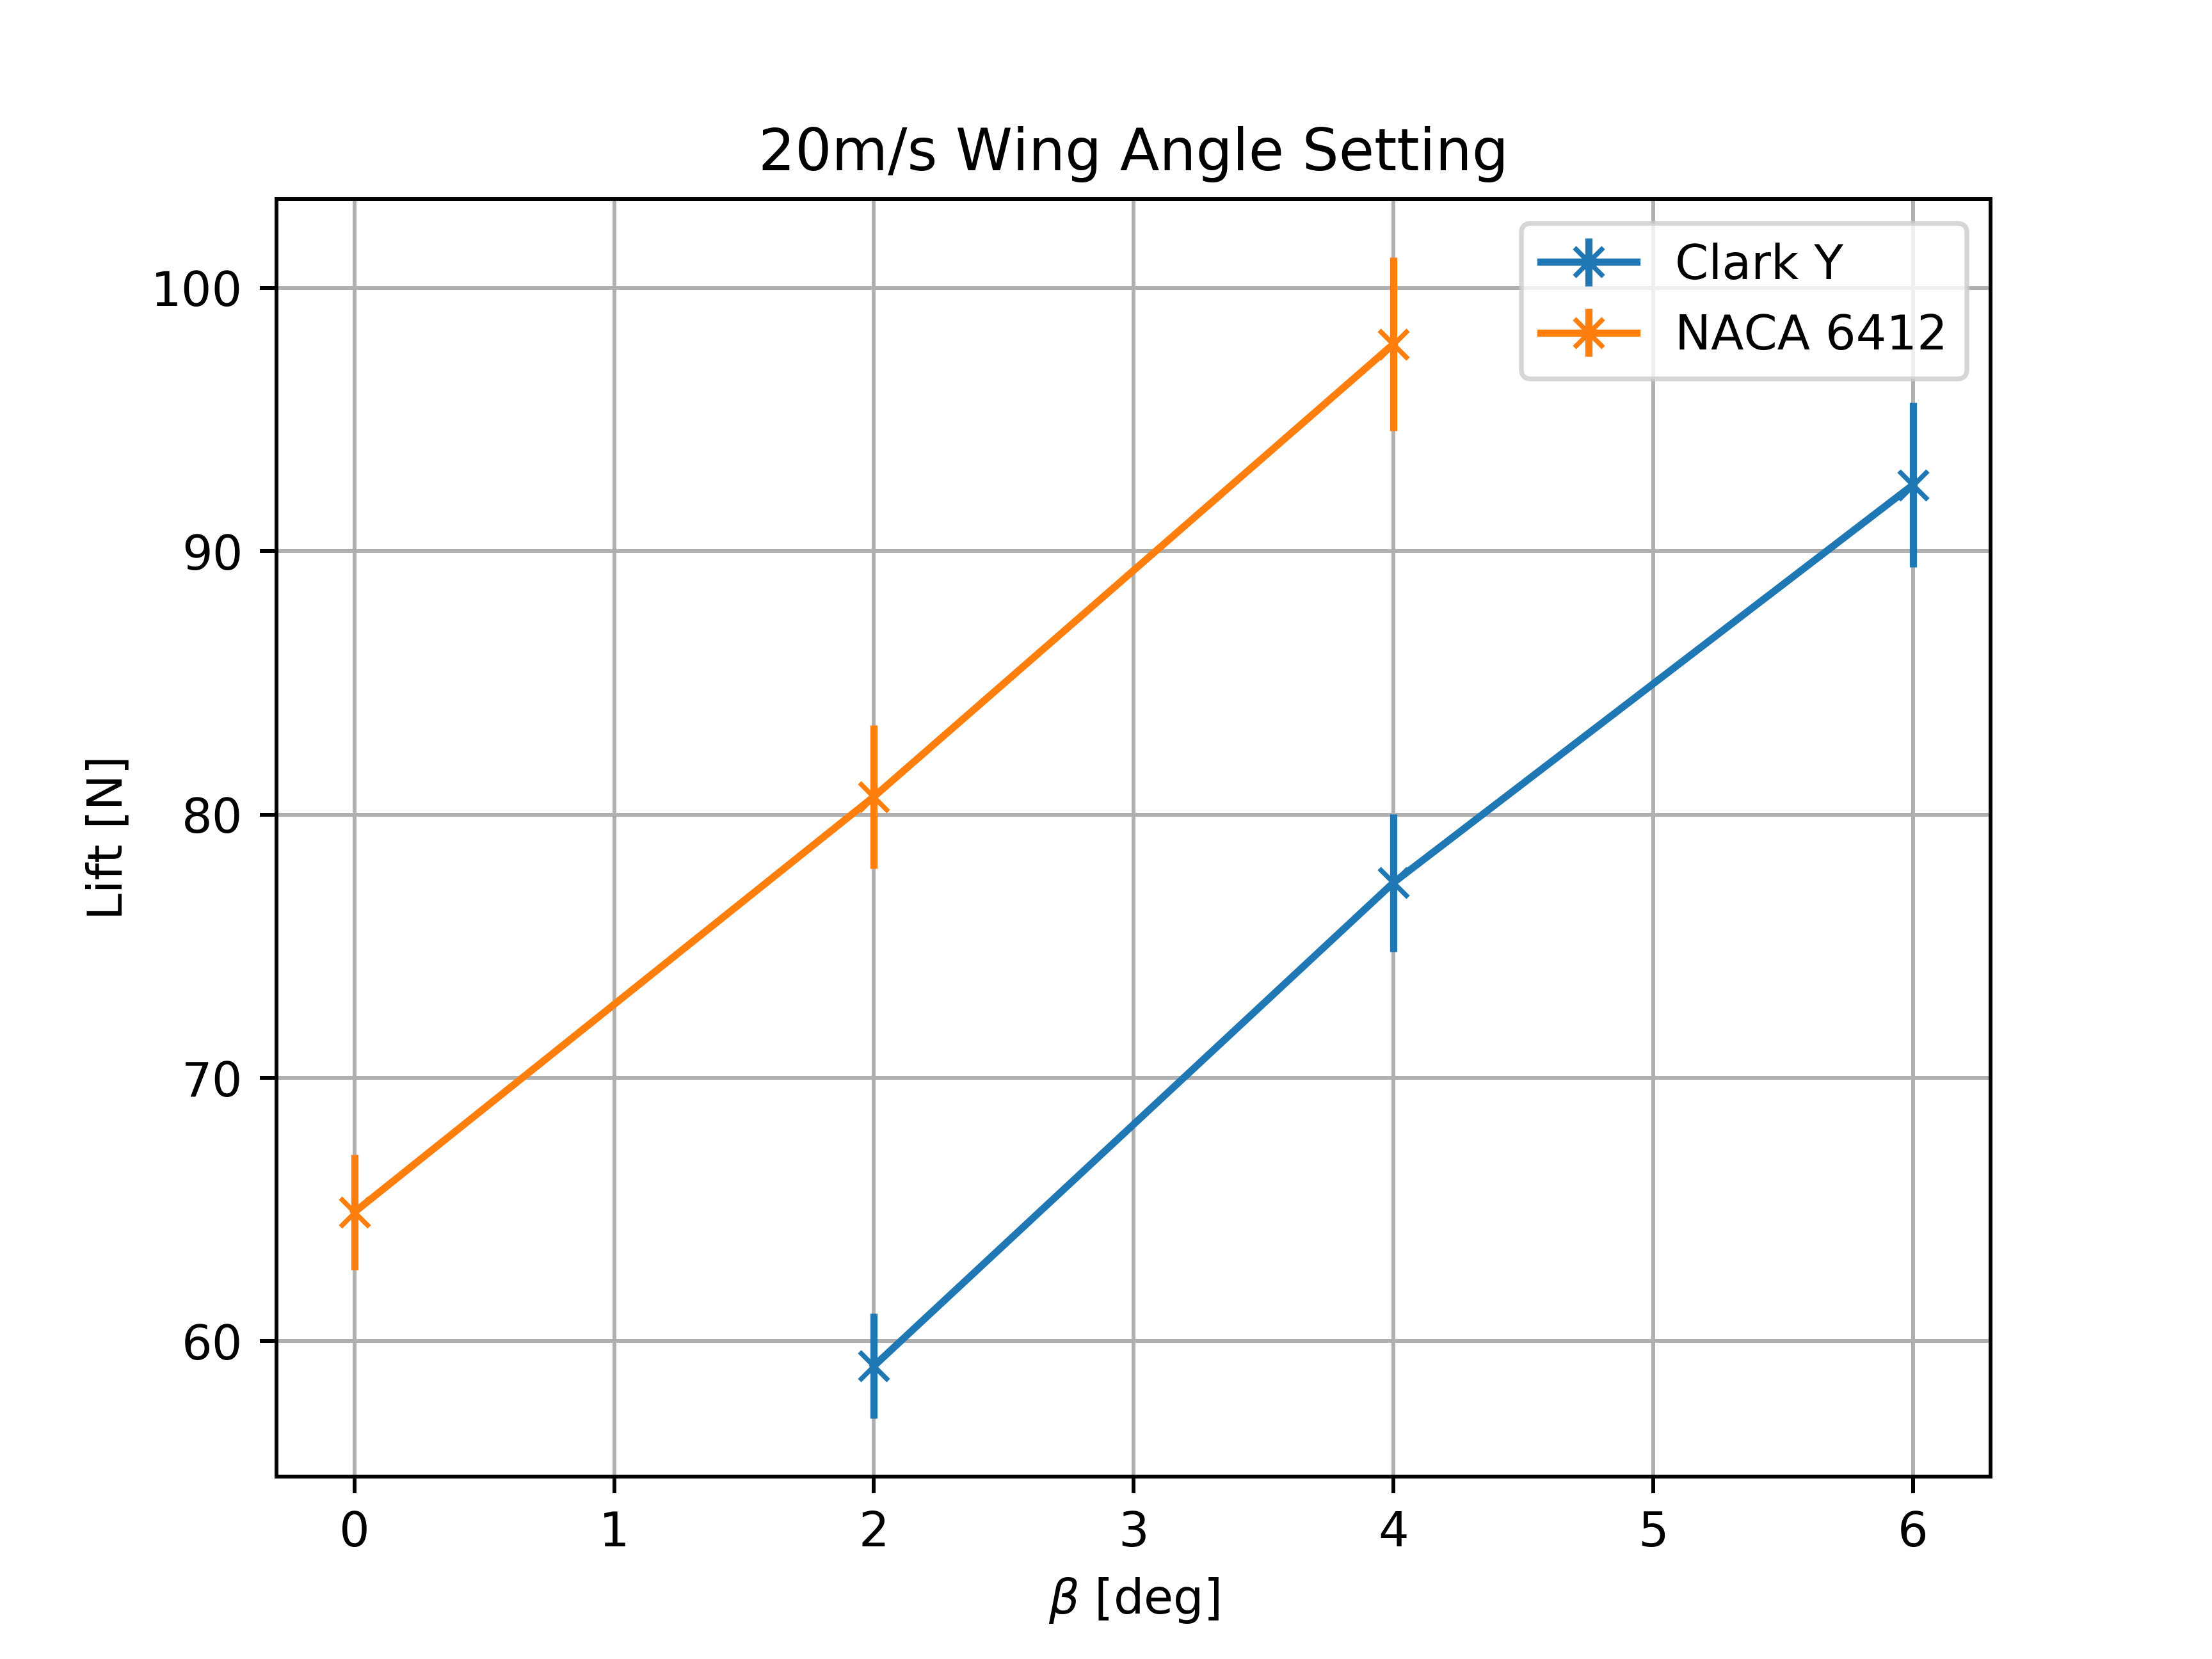
\includegraphics[width=\textwidth]{wing-setting-angle}
        \caption{Wing setting angle}
        \label{fig:wind-tunnel-results:wing-setting-angle}
    \end{subfigure}
    \hfill
    \begin{subfigure}[b]{0.49\columnwidth}
        \centering
        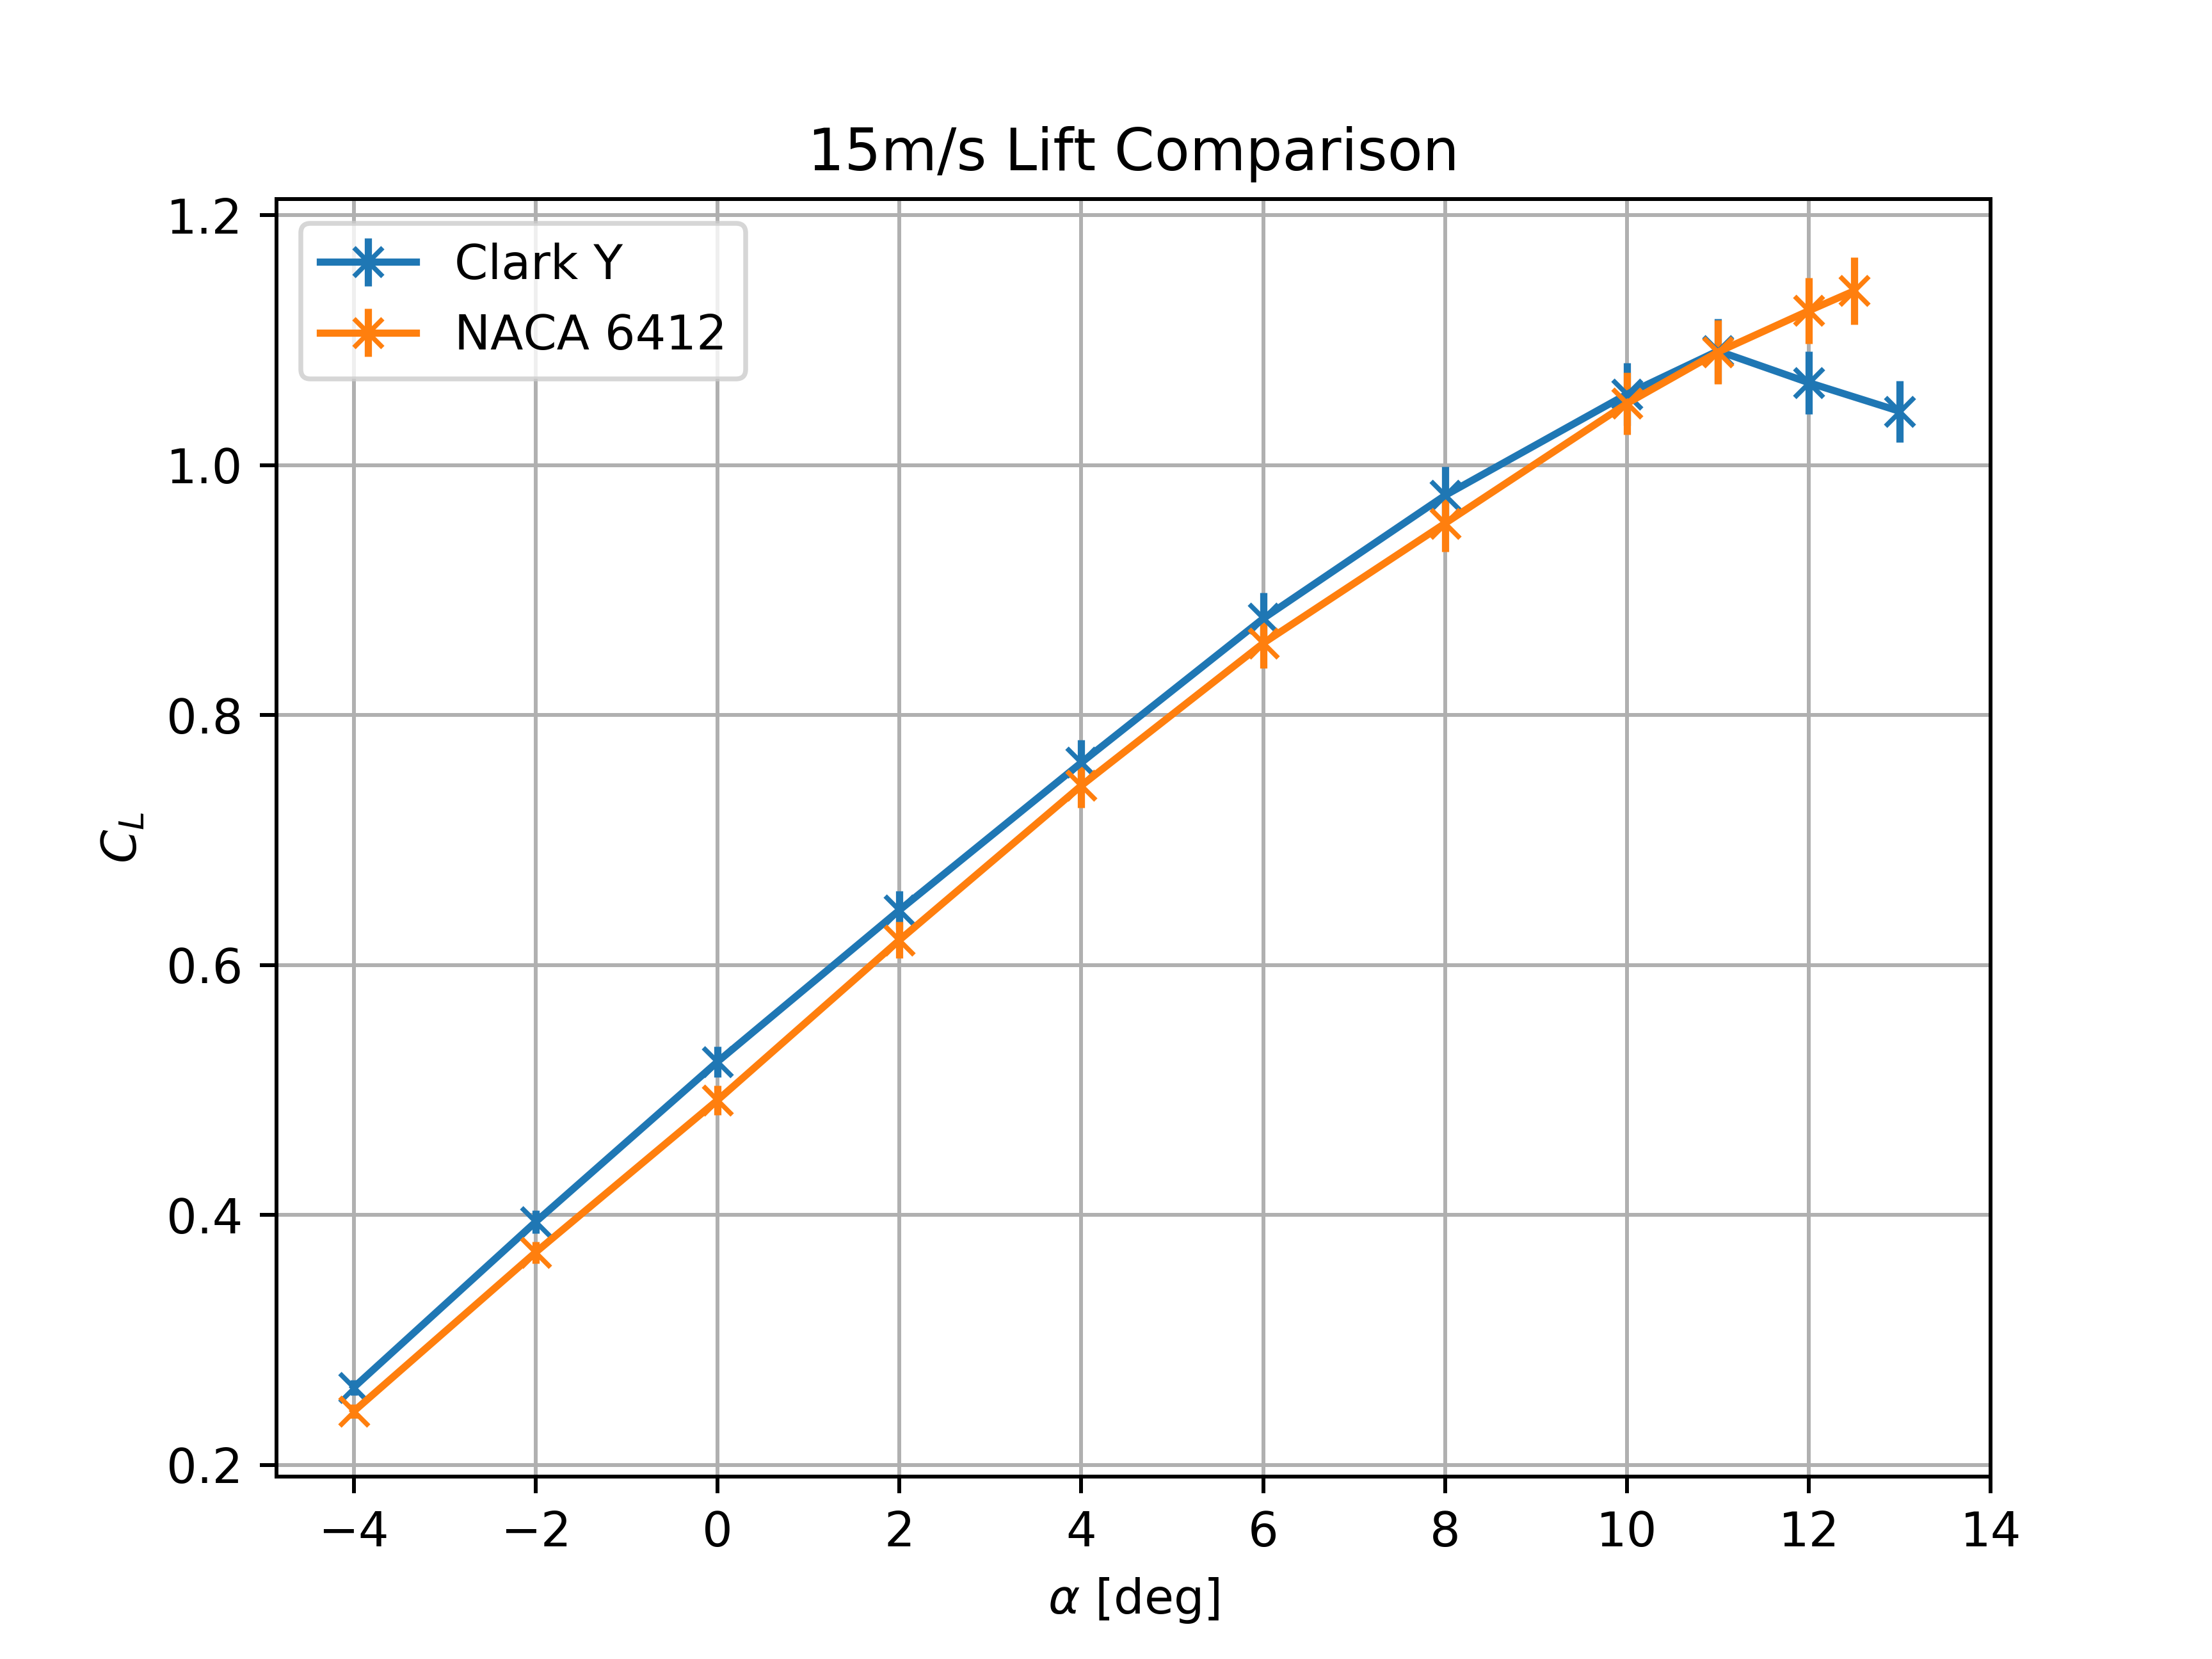
\includegraphics[width=\textwidth]{lift-comparison}
        \caption{Lift comparison}
        \label{fig:wind-tunnel-results:lift-comparison}
    \end{subfigure}

    \begin{subfigure}[b]{0.49\columnwidth}
        \centering
        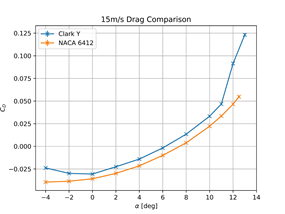
\includegraphics[width=\textwidth]{drag-comparison}
        \caption{Drag comparison}
        \label{fig:wind-tunnel-results:drag-comparison}
    \end{subfigure}
    \hfill
    \begin{subfigure}[b]{0.49\columnwidth}
        \centering
        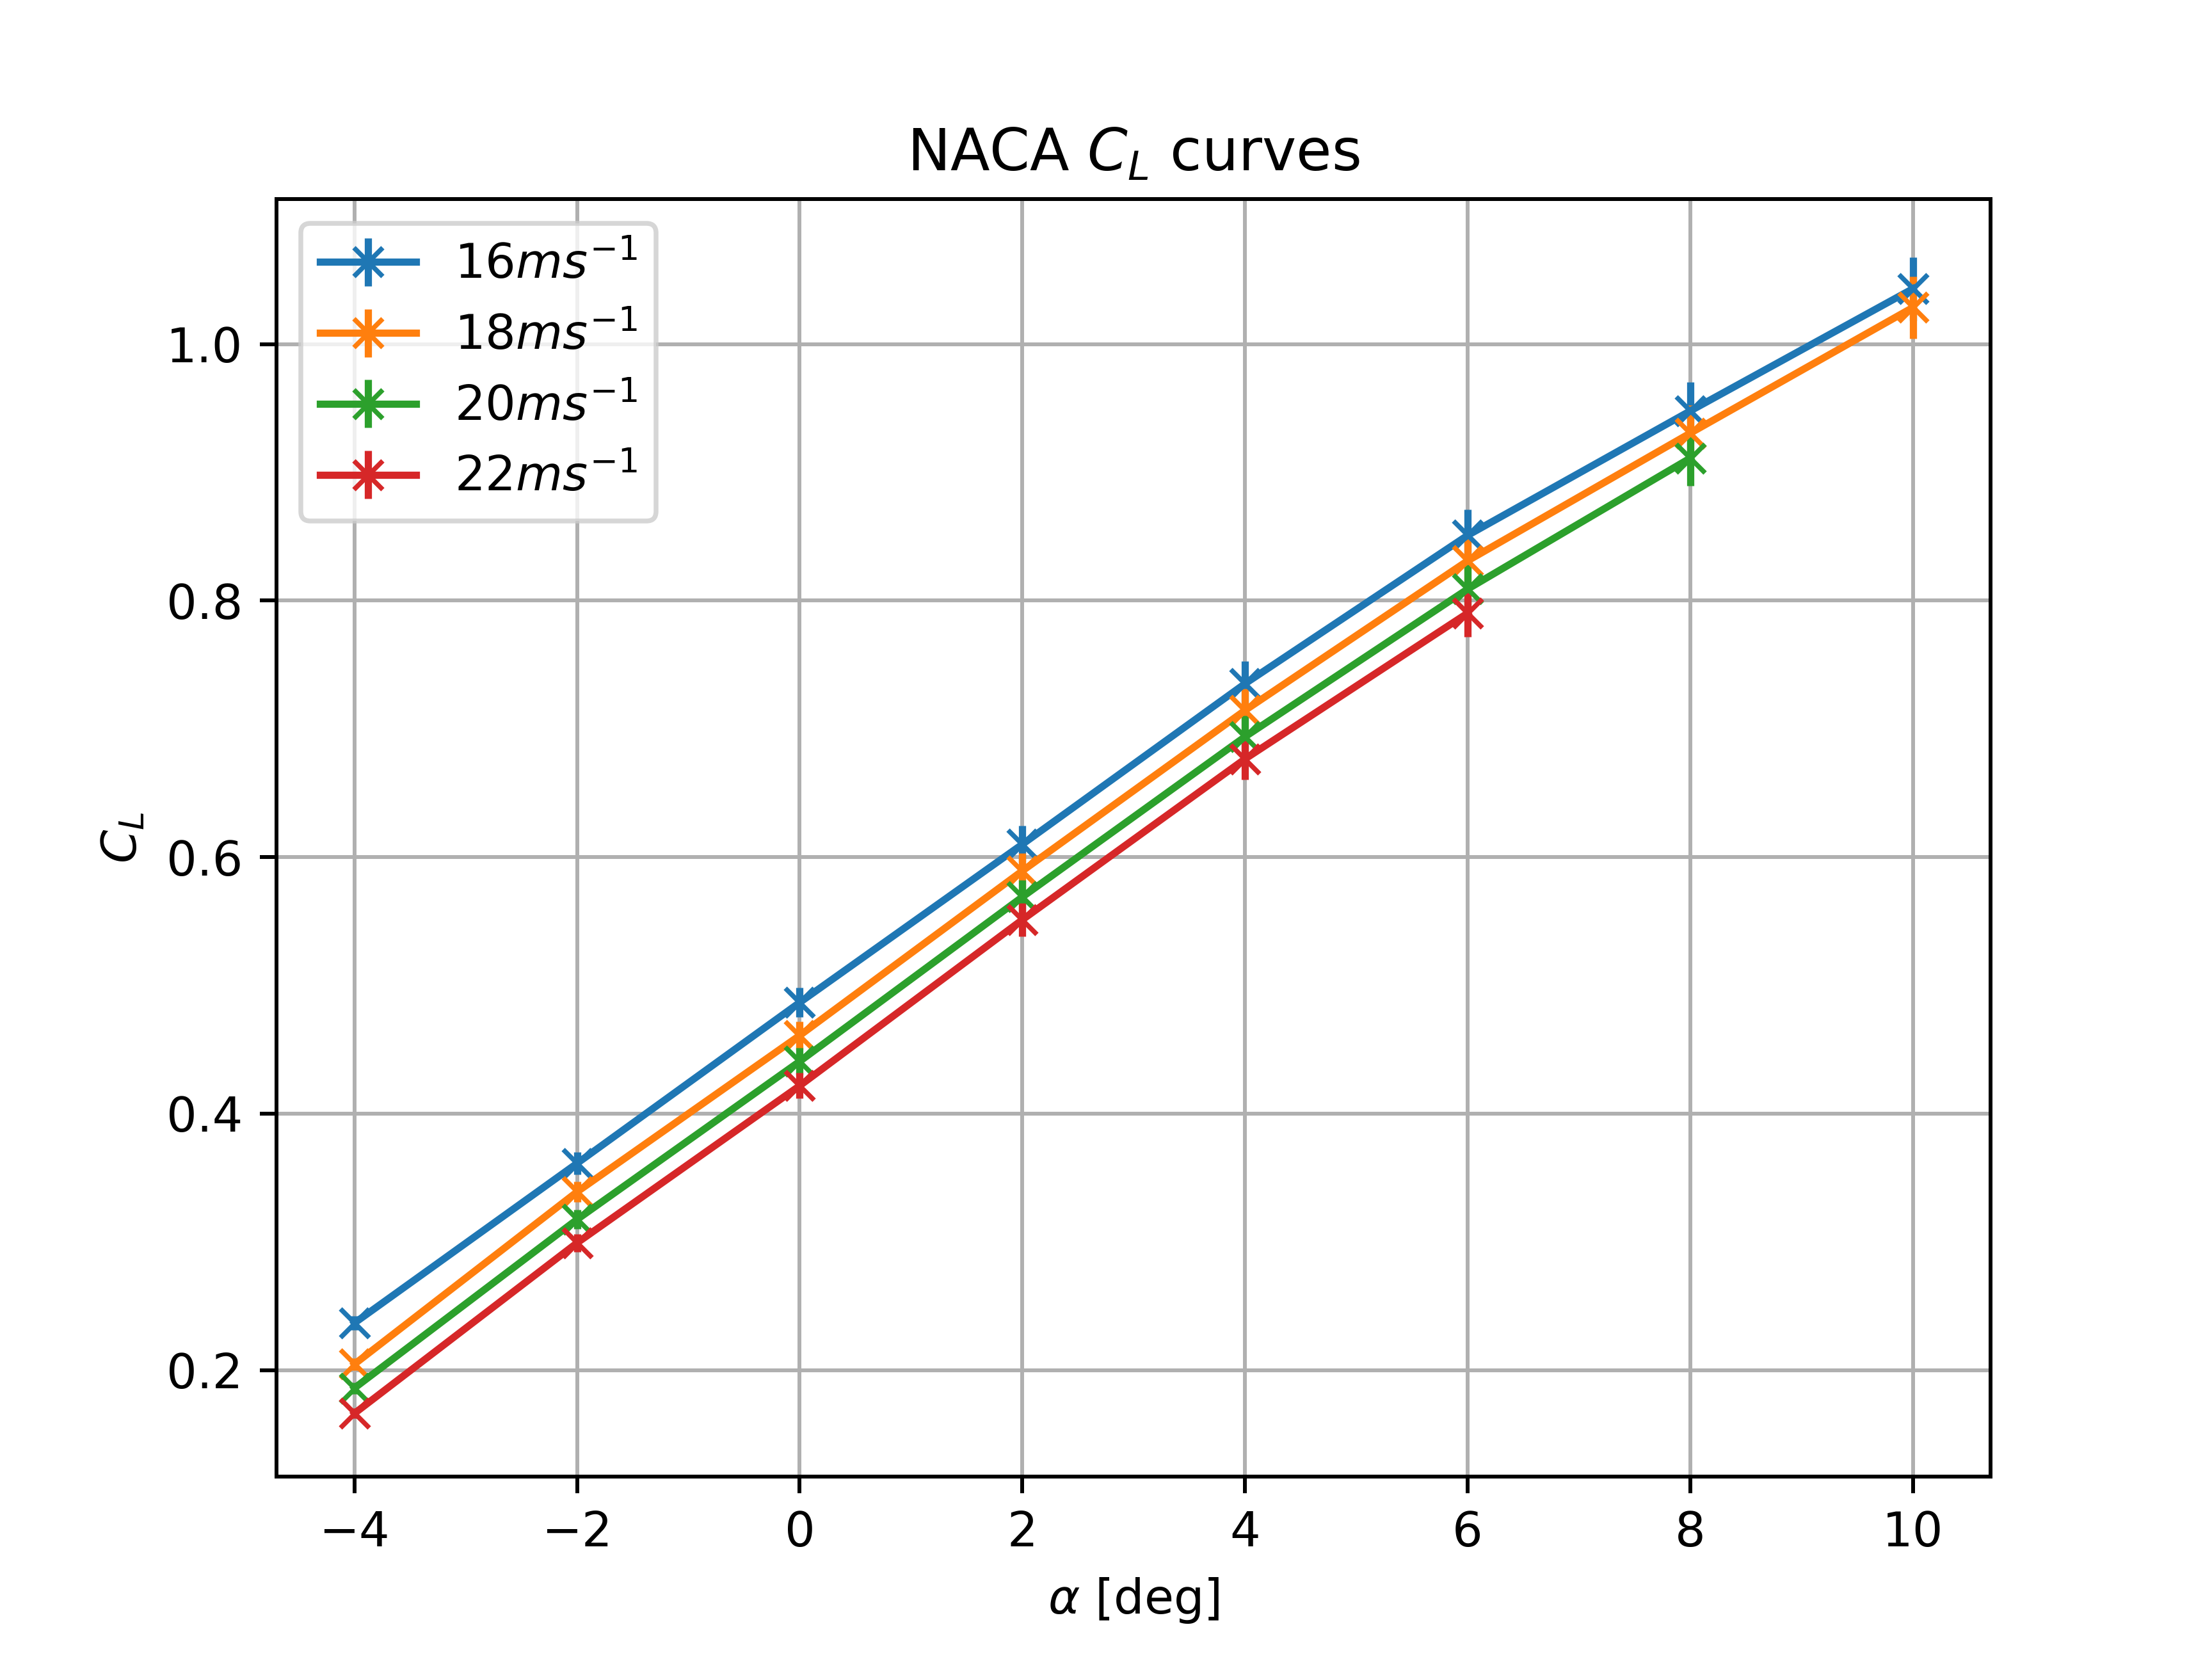
\includegraphics[width=\textwidth]{naca-lift-coefficient}
        \caption{NACA lift coefficient}
        \label{fig:wind-tunnel-results:naca-lift-coefficient}
    \end{subfigure}

    \begin{subfigure}[b]{0.49\columnwidth}
        \centering
        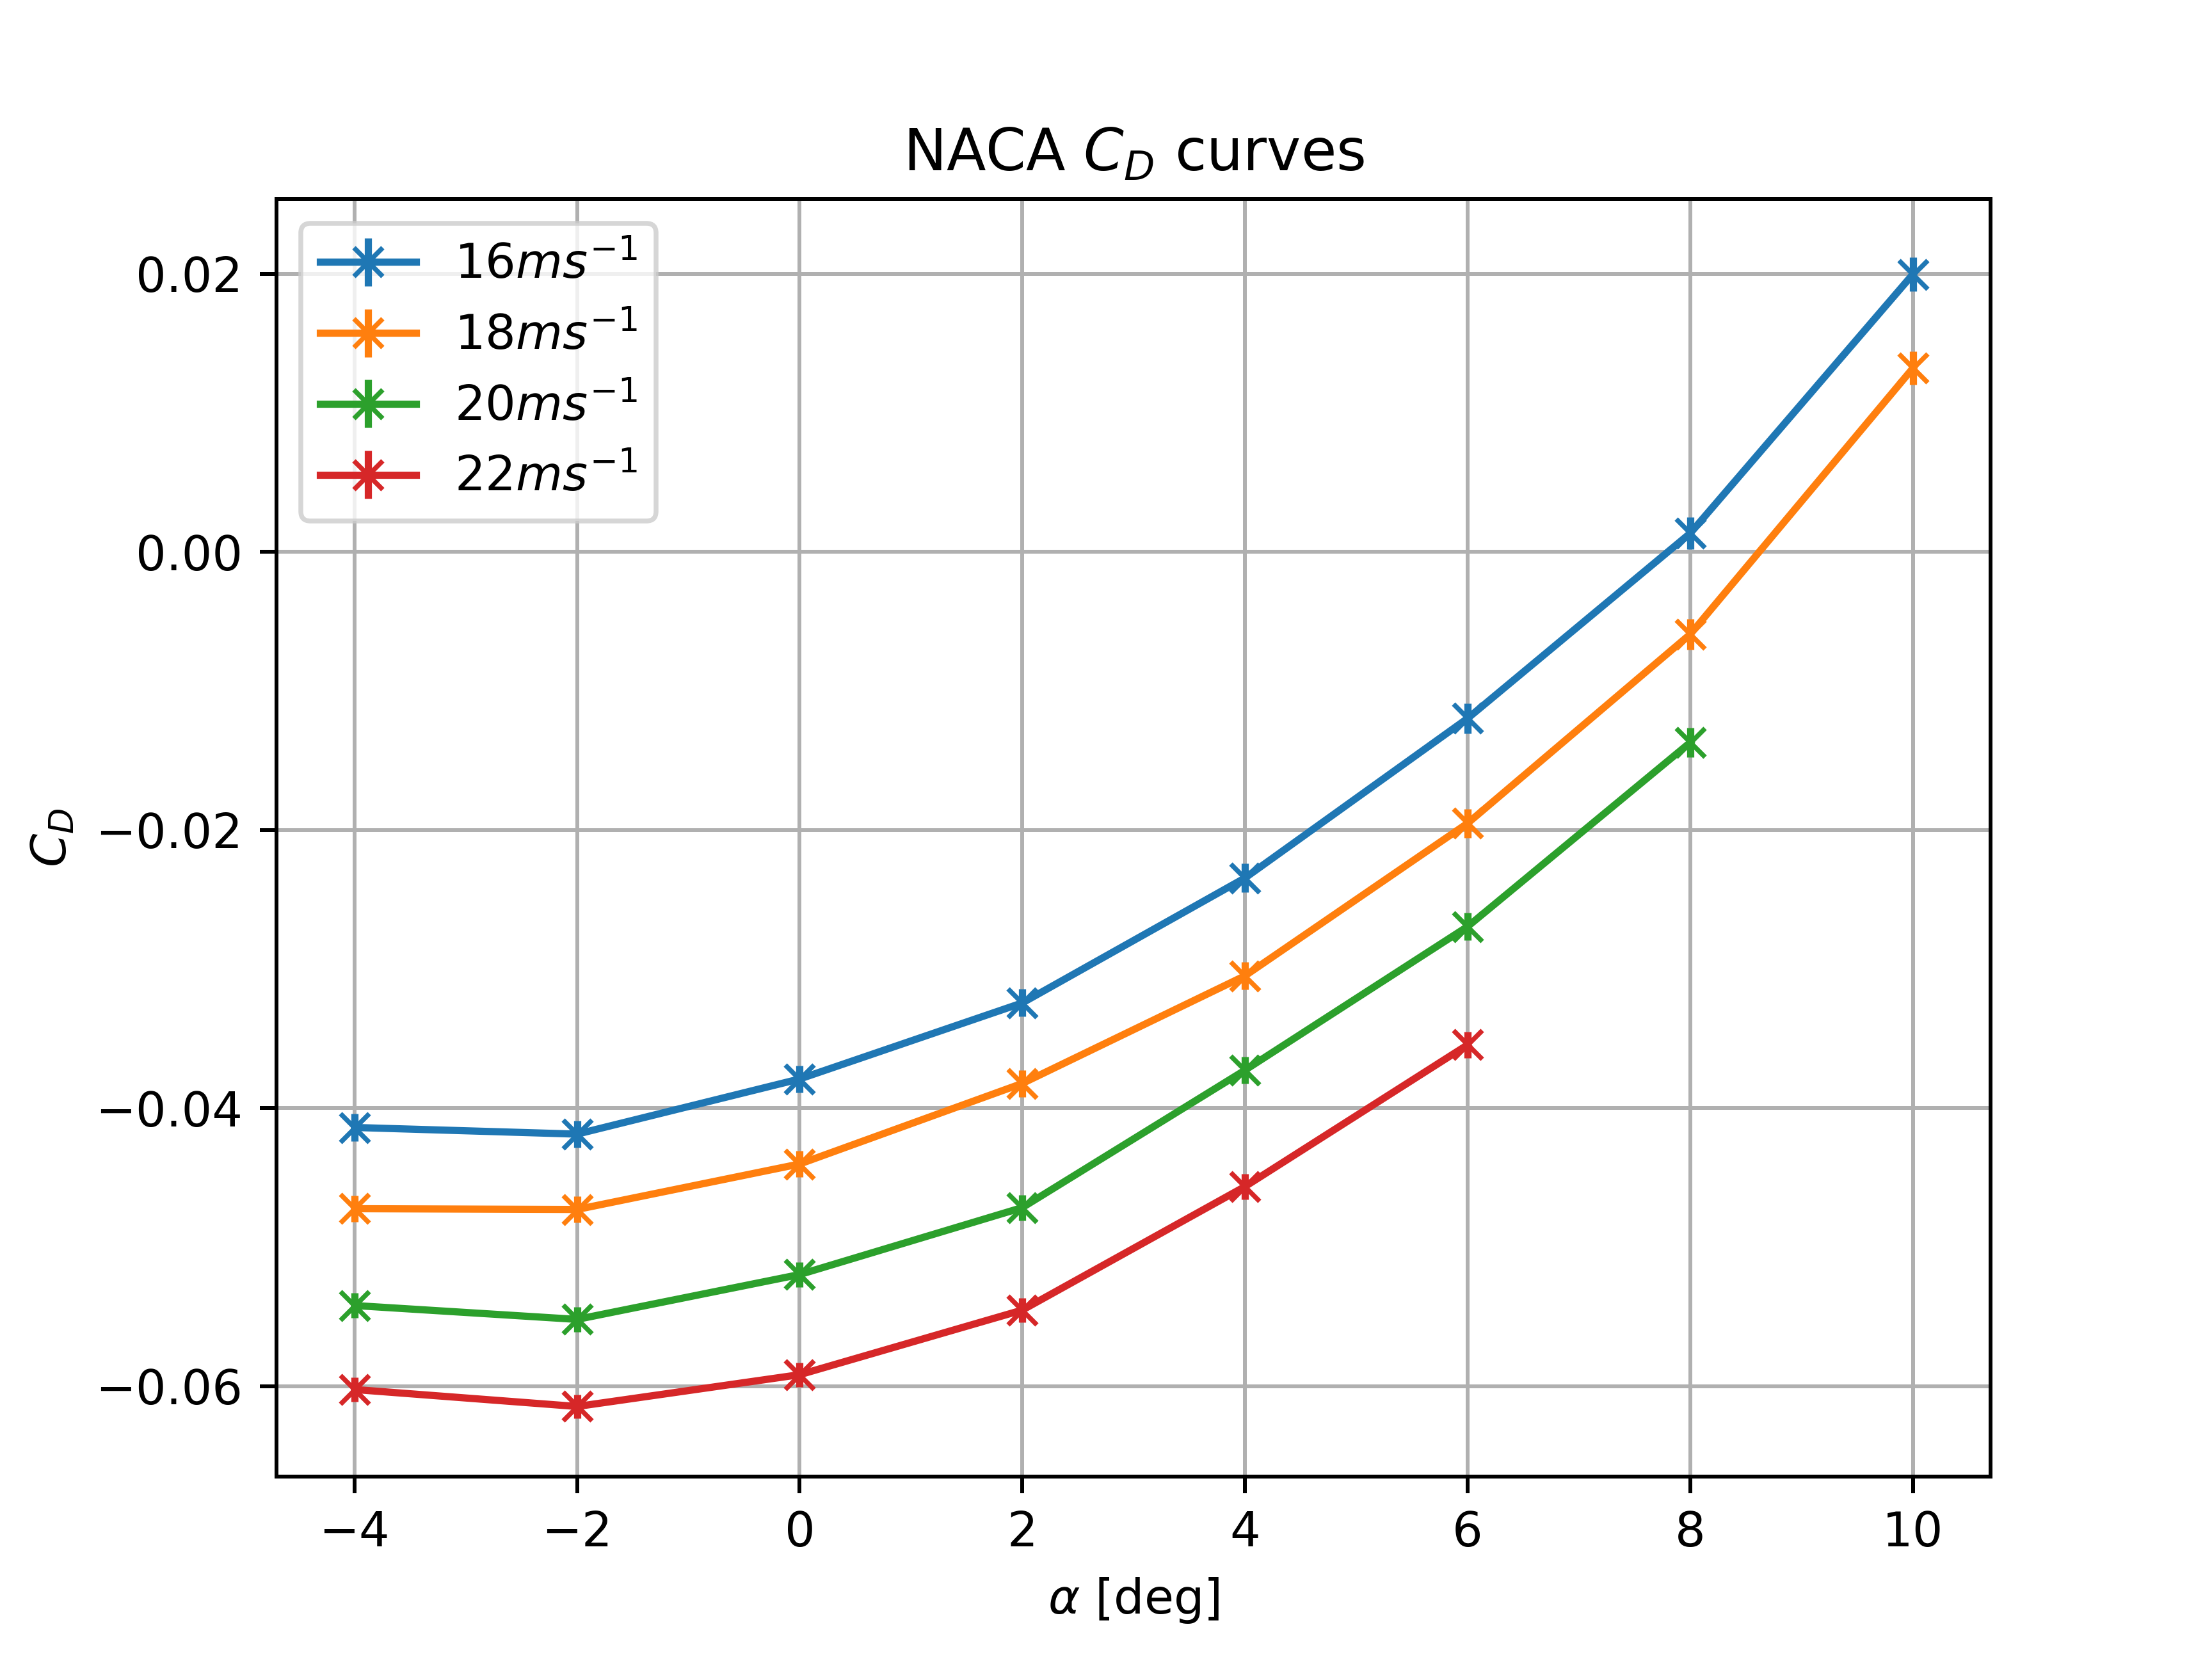
\includegraphics[width=\textwidth]{naca-drag-coefficient}
        \caption{NACA drag coefficient}
        \label{fig:wind-tunnel-results:naca-drag-coefficient}
    \end{subfigure}
    \hfill
    \begin{subfigure}[b]{0.49\columnwidth}
        \centering
        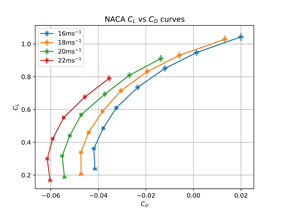
\includegraphics[width=\textwidth]{cl-against-cd}
        \caption{\cl\, against \cd}
        \label{fig:wind-tunnel-results:cl-against-cd}
    \end{subfigure}

    \begin{subfigure}[b]{0.49\columnwidth}
        \centering
        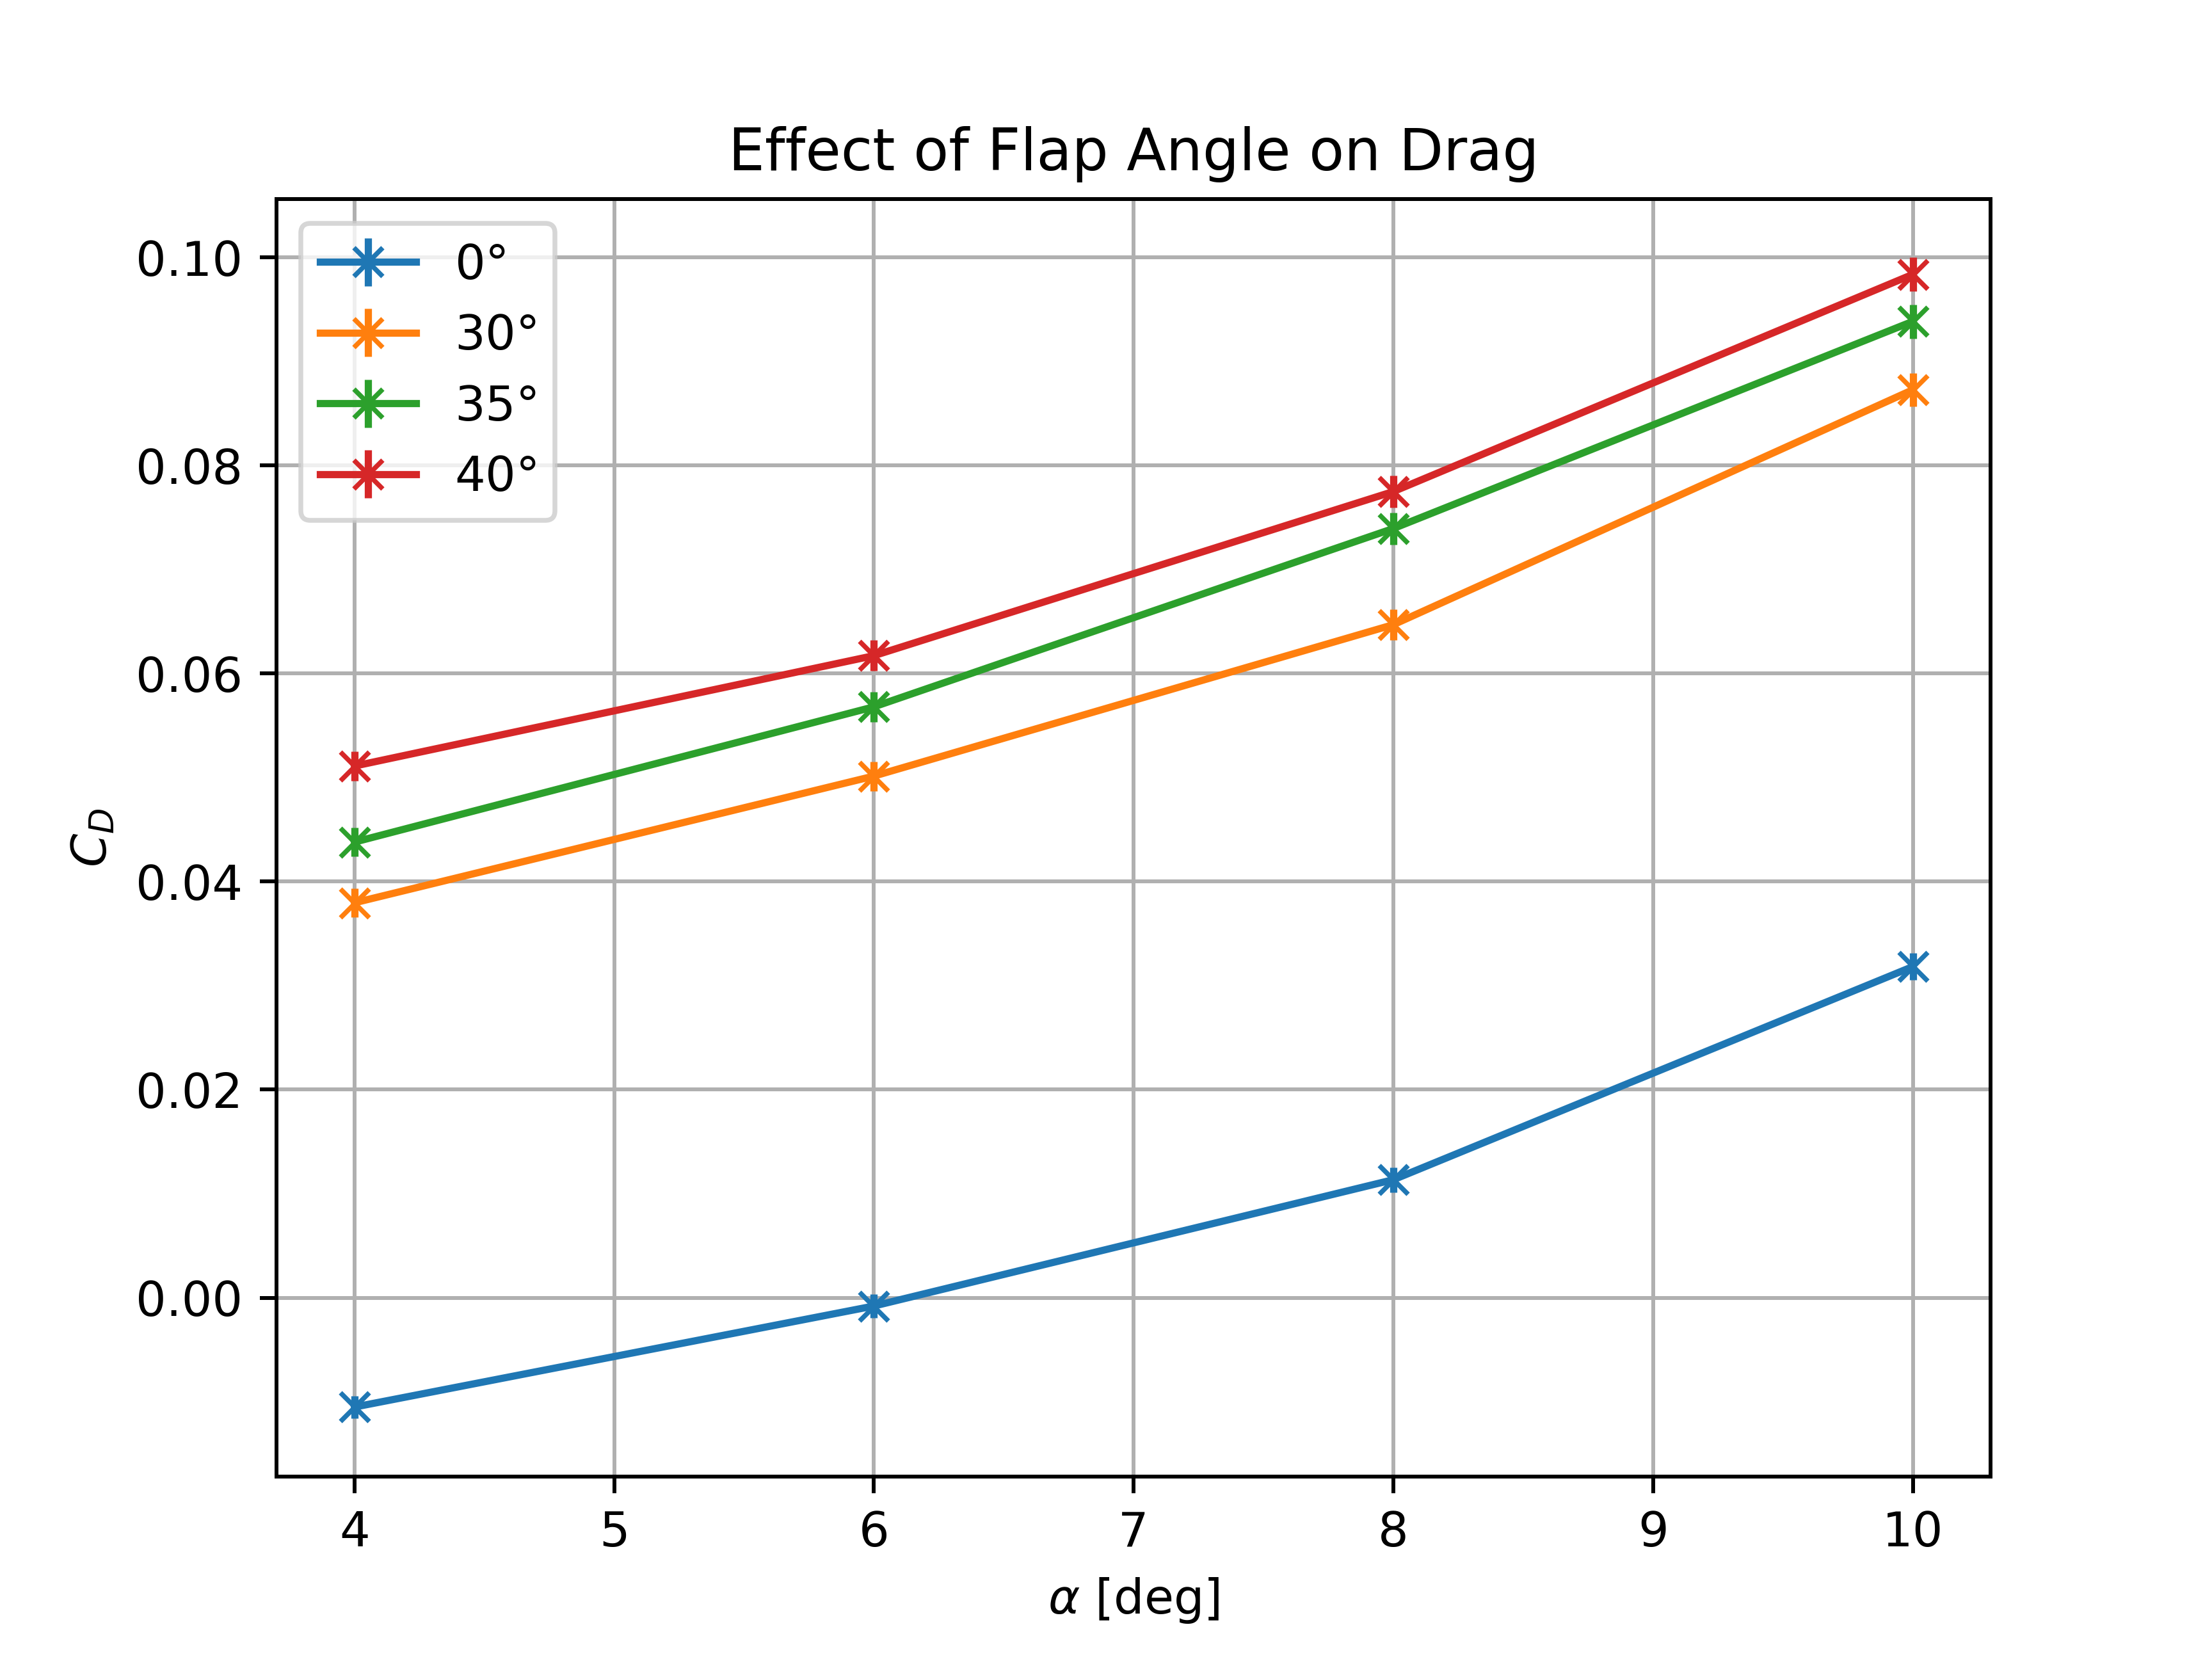
\includegraphics[width=\textwidth]{flap-drag-comparison}
        \caption{Flap drag comparison}
        \label{fig:wind-tunnel-results:flap-drag-comparison}
    \end{subfigure}
    \hfill
    \begin{subfigure}[b]{0.49\columnwidth}
        \centering
        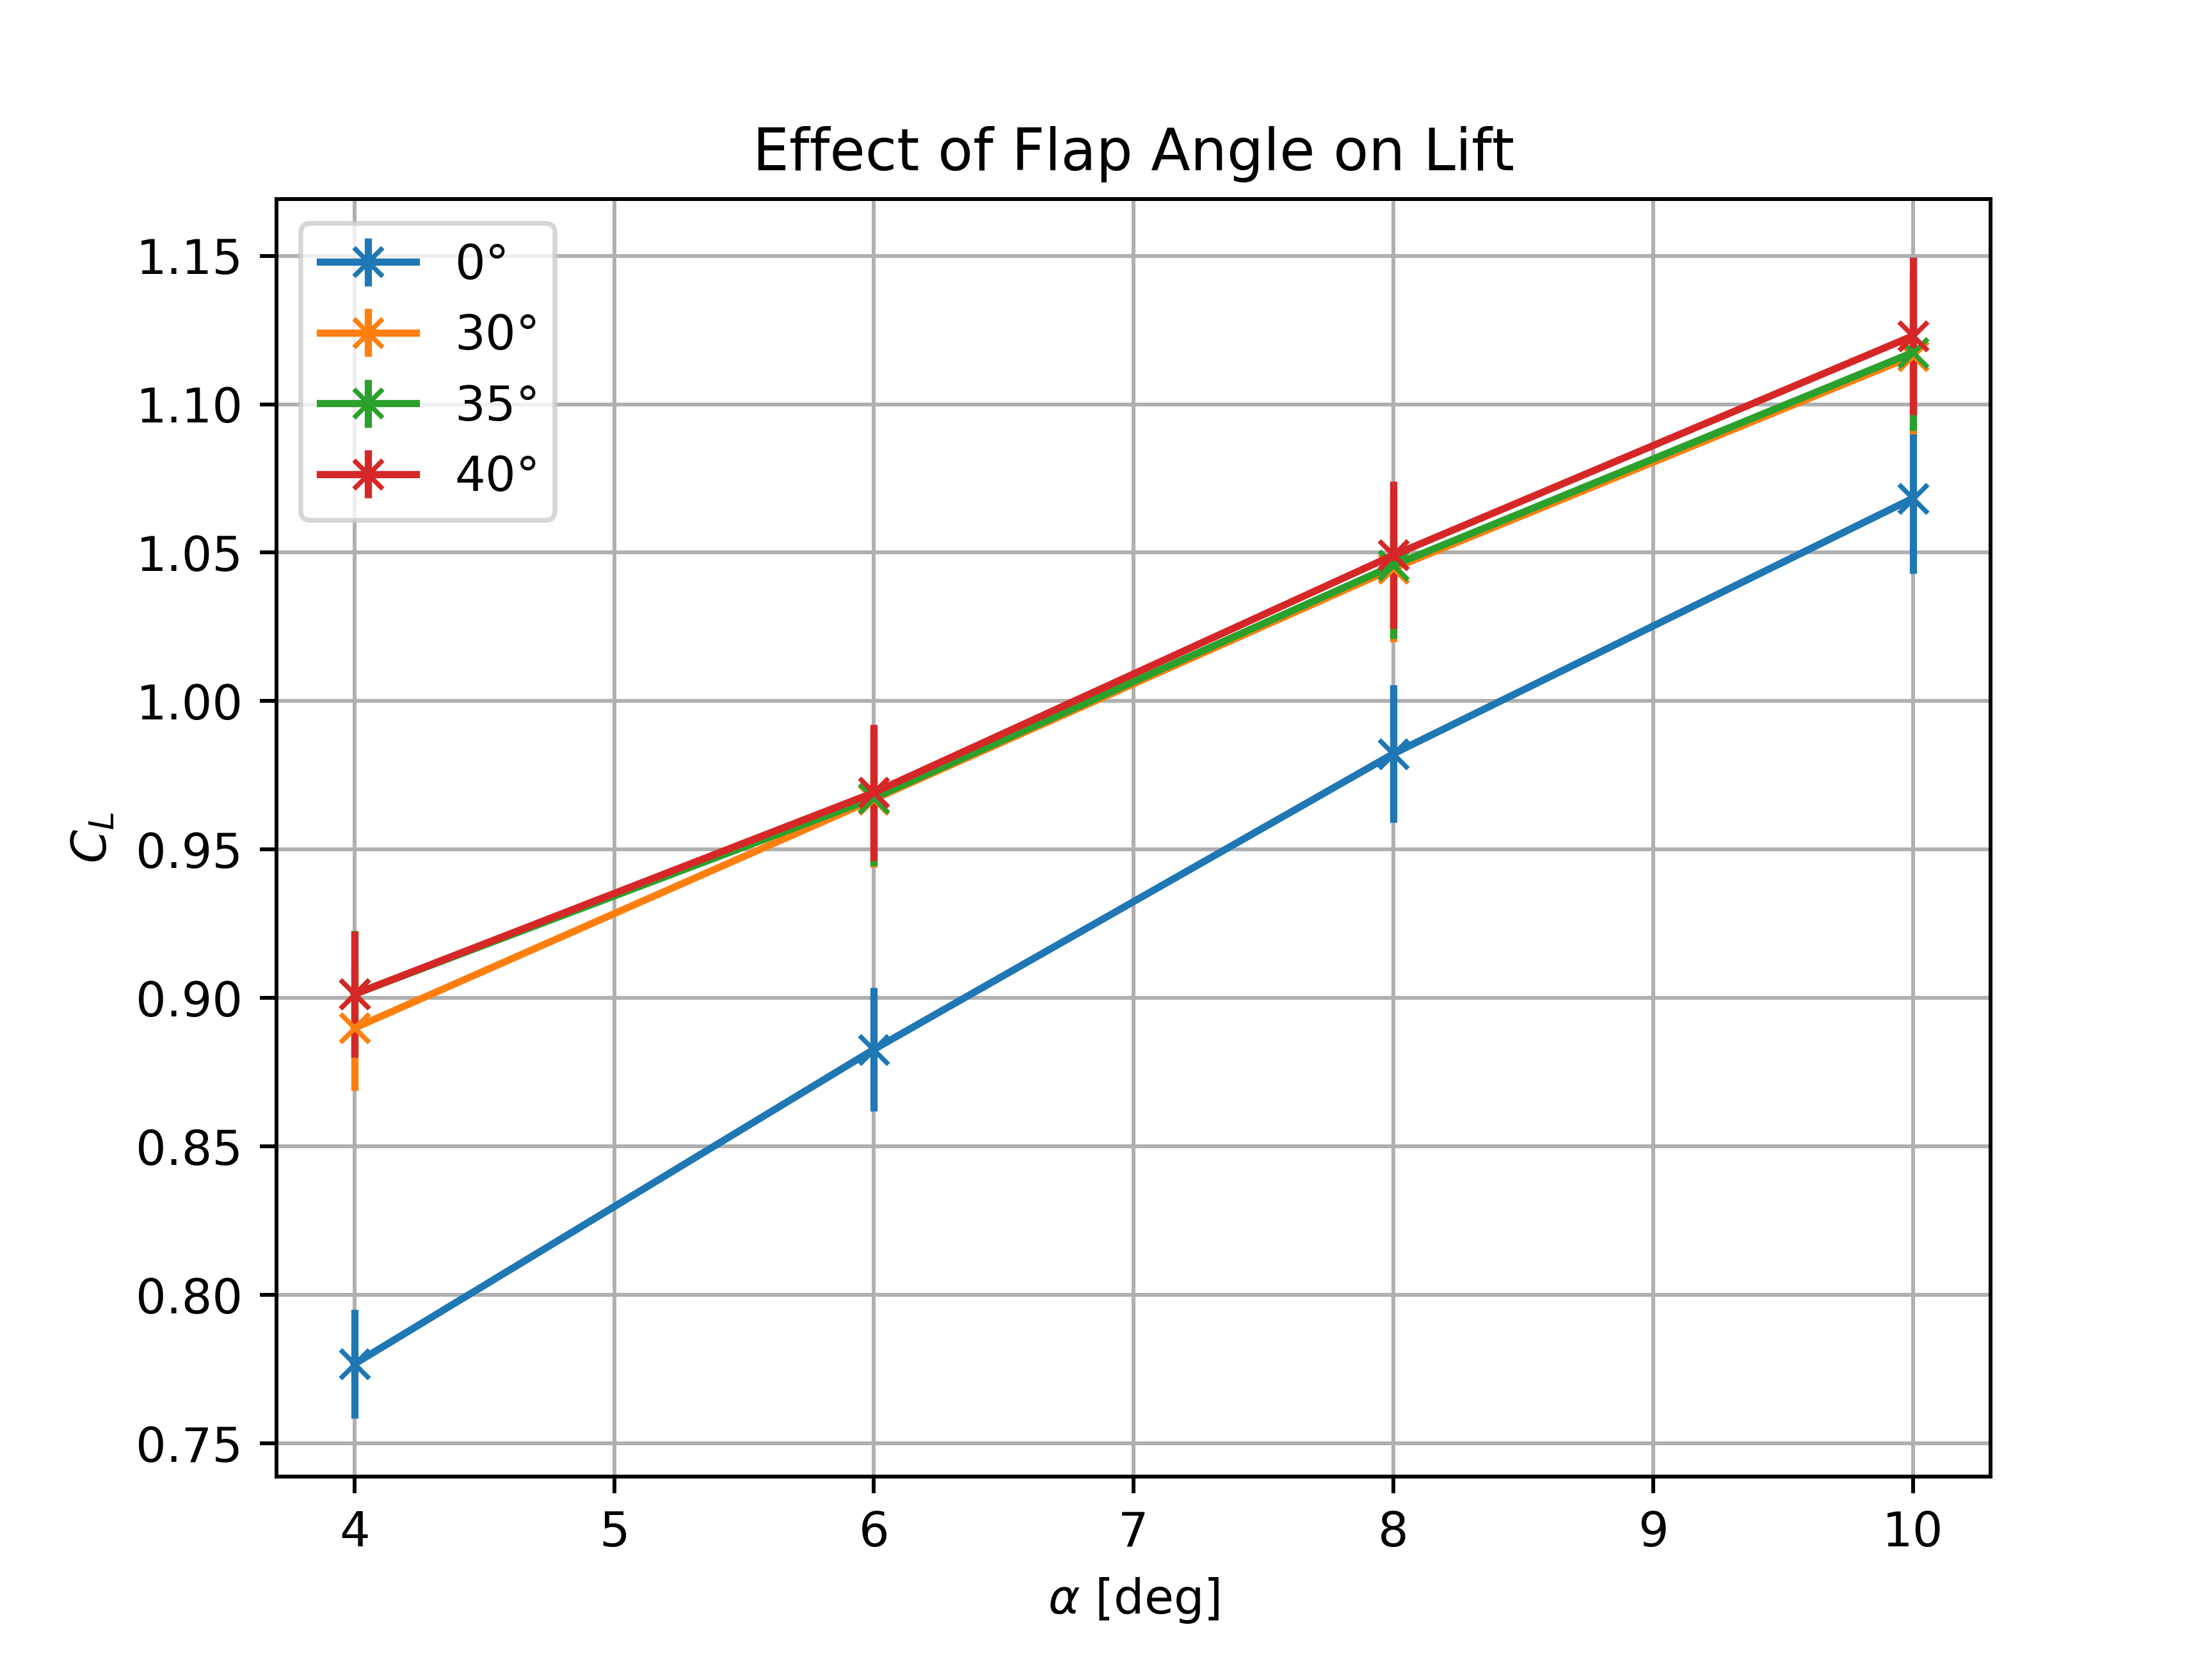
\includegraphics[width=\textwidth]{flap-lift-comparison}
        \caption{Flap lift comparison}
        \label{fig:wind-tunnel-results:flap-lift-comparison}
    \end{subfigure}

    \begin{subfigure}[b]{0.49\columnwidth}
        \centering
        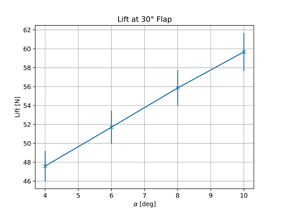
\includegraphics[width=\textwidth]{30-degree-flap-lift}
        \caption{30$^o$ flap lift}
        \label{fig:wind-tunnel-results:30-degree-flap-lift}
    \end{subfigure}
    \hfill
    \begin{subfigure}[b]{0.49\columnwidth}
        \centering
        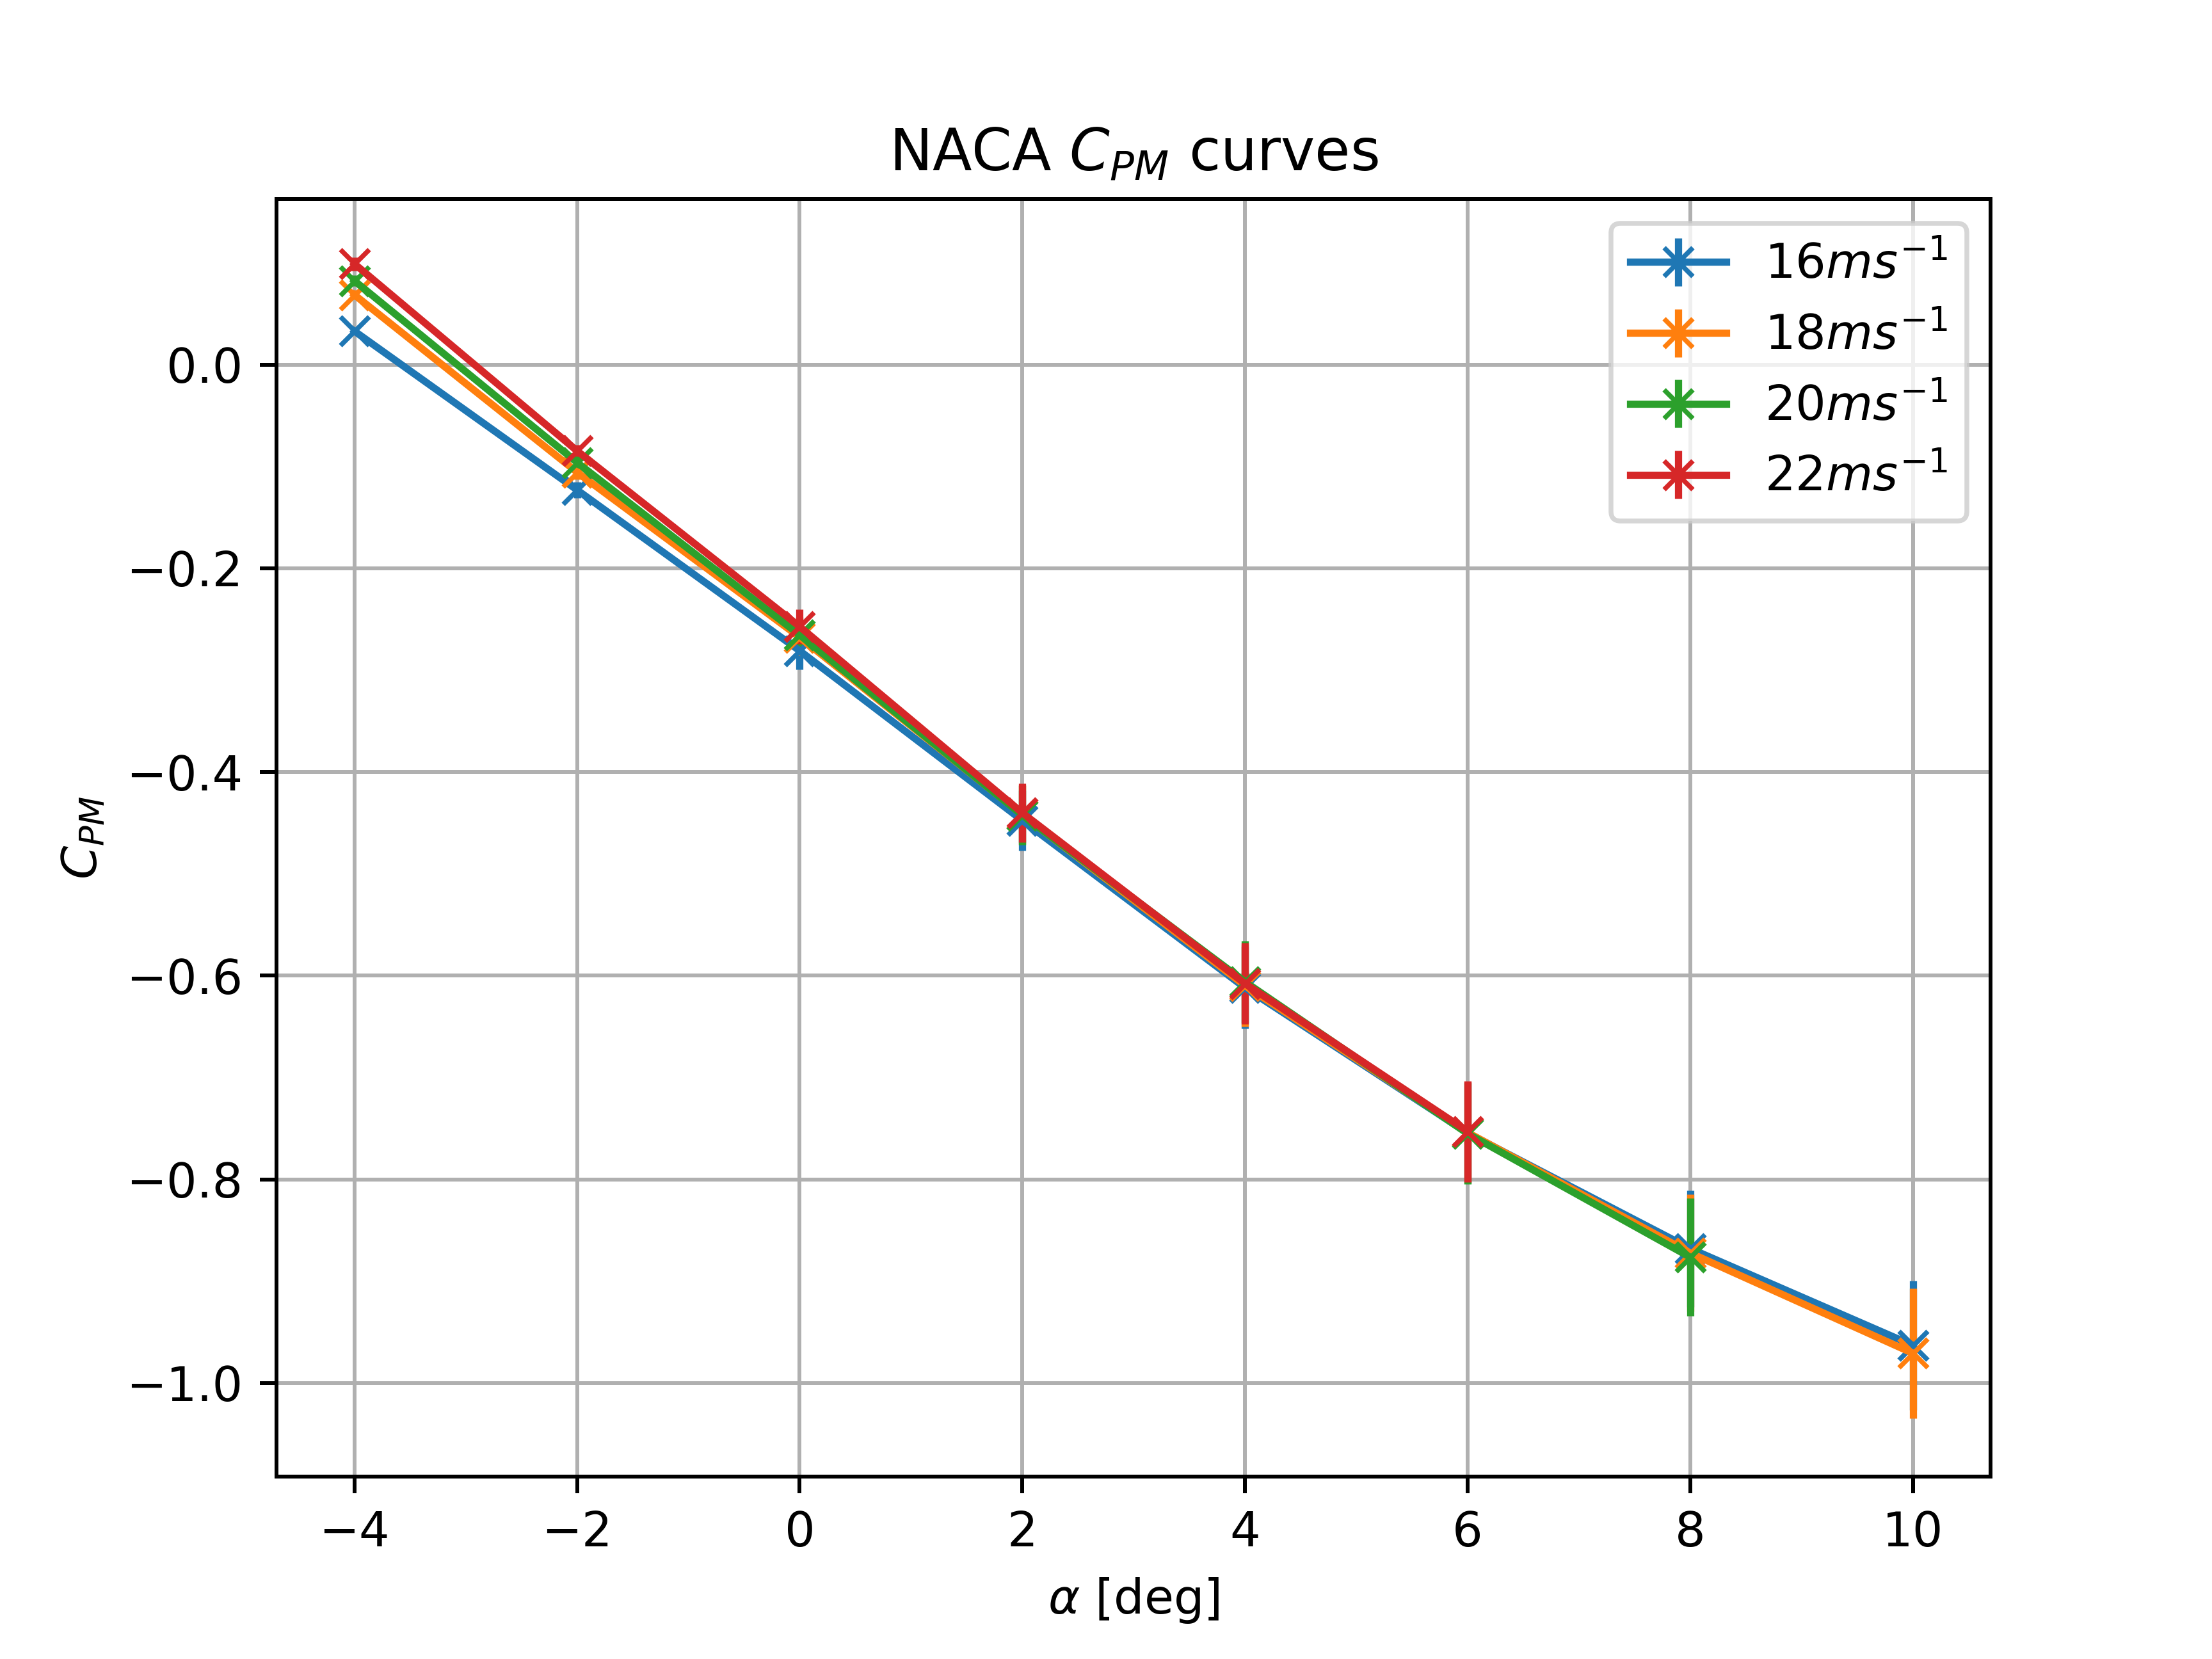
\includegraphics[width=\textwidth]{moment-coefficients}
        \caption{Moment coefficients}
        \label{fig:wind-tunnel-results:moment-coefficients}
    \end{subfigure}

    \caption{graphical results of the analysis of data gathered during the wind tunnel test.}
    \label{fig:wind-tunnel-results}
\end{figure}

The results from the wind tunnel test required considerable post-processing before analysis could be carried out, but once this was complete the graphs could be made and the results easily analysed.
There was a significant problem when the correction for the drag of the mounting structure, used to hold the model in the wind tunnel, was implemented because it caused some of the drag results to be negative.
The drag data were therefore unreliable, but the trends seen in the results could still be useful.
The drag data will now rely on CFD and additional wind tunnel tests for clarification.

Figure \ref{fig:wind-tunnel-results:wing-setting-angle} shows the results from the initial test carried out, where the setting angle of the two wings were found by increasing the angle of the wing against the fuselage until the lift exceeded the target weight of \newtons{70} at the target cruise speed of \mps{20}.
This graph shows that the NACA6412 exceeded this lift at \degr{1}, and so was set at \degr{2} for the rest of the test to give a margin as the final wing is expected to produce slightly less lift due to the attachment of the propulsion units.
The Clark Y exceeded the required lift at around \degr{3} and so was set at \degr{4} for the same reason. 

Figures \ref{fig:wind-tunnel-results:lift-comparison} and \ref{fig:wind-tunnel-results:drag-comparison} show the comparison between the NACA6412 and Clark Y wings through a full sweep of angle of attack.
At this point the wings were set at their optimal angles, and so the whole model was moved through the range of angles of attack to give the data.
It can be seen that the two wings produce very similar \cl\, values; while this is expected since the wings are set at their optimal angles, the Clark Y aerofoil stalls before the NACA6412, thus giving a lower maximum lift.
This is one of the reasons the NACA6412 was chosen as the aerofoil for the final UAV instead of the Clark Y.
It can also be seen that the Clark Y has a higher \cd\, at all angles of attack, and so is less efficient than the NACA6412.

Figures \ref{fig:wind-tunnel-results:naca-lift-coefficient} through \ref{fig:wind-tunnel-results:cl-against-cd} show the plots for the wind tunnel model equipped with the NACA6412 at a range of airspeeds, showing the performance throughout the target flight envelope of the UAV.
Figure \ref{fig:wind-tunnel-results:naca-lift-coefficient} shows that the \cl\, remains almost constant as the airspeed changes and that, as expected, there are no compressibility effects as these speeds.
Figure \ref{fig:wind-tunnel-results:naca-drag-coefficient} shows that the \cd\, reduces with the increase in airspeed, which is due to the reduction of lift induced drag at higher speeds.
Figure \ref{fig:wind-tunnel-results:cl-against-cd} shows that the highest aerodynamic efficiency is therefore found at the highest tested speed of \mps{22}, and although this speed is above the targeted cruise speed of the UAV, one can conclude that to maximise range the UAV should be flown as fast as possible. 

Figures \ref{fig:wind-tunnel-results:flap-drag-comparison} and \ref{fig:wind-tunnel-results:flap-lift-comparison} show the results of the flap test that was performed with the NACA6412 wing.
Figure \ref{fig:wind-tunnel-results:flap-drag-comparison} shows the increase in \cd\, that comes with each increment of the flap angle, while Figure \ref{fig:wind-tunnel-results:flap-lift-comparison} shows that the \cl\, increases significantly with the flaps activated but that the variation of the flap angle has little to no effect on the increase in \cl.
This suggests that the flaps are stalling at \degr{30}, and so the flap angle to be used in the final model was chosen to be \degr{30}.
Figure \ref{fig:wind-tunnel-results:30-degree-flap-lift} shows that the lift increase was not enough to provide the required lift at the target takeoff and landing speed of \mps{12}, with the maximum lift produced being just under \newtons{60} at \degr{10}.
The wing had not stalled at this point and so there was the possibility that the wing could produce more lift at a higher angle of attack, though this could not be tested as \degr{10} was the highest wing-body angle that could be reached.
Even so, it became clear that the design of the flaps needed to be modified to improve their effectiveness, and also that the area of the wing used for the flaps should be increased in order to maximise their effectiveness. 

The wind tunnel test also provided data for the pitching moment about the aerodynamic centre of the wing, as shown in Figure \ref{fig:wind-tunnel-results:moment-coefficients}, which gives an insight into the aerodynamic stability of the model and the pitching moment developed by the wing.
The data show that the coefficient of pitching moment is independent of airspeed is negative at \degr{0} angle of attack, which is less than ideal since it implies that the aircraft would want to pitch down, requiring the pilot to trim the model or use constant elevator in order to fly level.
The negative gradient of the line on the plot is good, however, as it implies that the aircraft is aerodynamically statically stable in pitch, so any pitching up of the aircraft would produce an increase in the pitching down moment and the aircraft would automatically stabilise.
Furthermore, with an adjustment to the tailplane, the magnitude of the pitching moment could be made zero at \degr{0} angle of attack by producing a counteracting moment with an angled tailplane, meaning that the pilot would not need to trim the aircraft to the same extent. 

The uncertainty of the results was calculated and is shown as vertical bars for every point on the plots in Figure \ref{fig:wind-tunnel-results}.
The uncertainties were calculated using the known accuracies of the recorded results, as well as repeats performed during the testing.
The maximum number of repeats for one test was only two, and so while the sample size is not significant, the uncertainties are still reasonably small even with a \pc{95.45} confidence.
These uncertainties were then converted to percentages and applied to all results of that type, with an example table for the uncertainty of \cl\, shown in Table \ref{tbl:cl-uncertainty}, and the others provided in Appendix \ref{appendix:unknown}.  % TODO: find appendix reference 

% TODO: units
% TODO: define uncertainty and variance outside table
% TODO: reduce width slightly
\importtable{|
    >{\raggedright\arraybackslash}m{0.16\columnwidth}
    >{\raggedleft\arraybackslash}m{0.16\columnwidth}
    >{\raggedleft\arraybackslash}m{0.17\columnwidth}
    >{\raggedleft\arraybackslash}m{0.17\columnwidth}
    >{\raggedleft\arraybackslash}m{0.17\columnwidth} |
}{
    \hline
    Measured variable & $L$ & $q$ & $S$ & Rep. \cl \\
    \hline
    Typical value & 77.04 & 249.55 & 0.6 & 0.01715 \\
    Accuracy & 0.07704 & 0.349 & 0.0012 & 0.01213 \\
    PDF & rect. & rect. & rect. & norm. \\
    PDF factor & 1.7321 & 1.7321 & 1.7321 & 1 \\
    $k$ factor & 1 & 1 & 1 & 1 \\
    SC value & 0.006679 & -0.00206 & -0.85754 & 1 \\
    Uncertainty & 0.000297 & -0.000416 & -0.000594 & 0.012128 \\
    Variance & $9\times10^{-8}$ & $1.7\times10^{-7}$ & $3.5\times10^{-7}$ & $1.471\times10^{-4}$ \\
    \hline
}{uncertainty calculations for \cl; the uncertainty and variance rows refer to the value of uncertainty and its variance in each measured variable.}{cl-uncertainty}

\importtable{| l r |}{
    \hline
    Combined standard uncertainty & 0.01215 \\
    \cl\, mean & 0.5145 \\
    Percentage uncertainty & 2.36 \\
    \hline
}{uncertainty summary for \cl.}{uncertainty-summary}

Unfortunately, the scope of the work required to design a fully functional tailplane with control surfaces had not yet been realised, and the design was far too simple, with no mounting angle or control surfaces.
The tail was also undersized, as observed by the project supervisors.
Because of this, little work went into analysing the results from this test in terms of the tailplane, and work on the next version essentially started from scratch. 

\subsection{Motor and propellor test} \label{sec:design-process:interim-design-review:motor-and-propellor-test}

\subsubsection{Overview} \label{sec:design-process:interim-design-review:motor-and-propellor-test:overview}

\importimage{motor-bracket}{the motor bracket attached to the rear of the motor.}{Motor bracket}{0.5}
\importimage{motor-test}{the motor in the wind tunnel.}{Motor test}{0.5}

Once the motor and propeller selection had been completed based on wind tunnel results and propeller performance analysis, one of the wing motors was ordered with its tractor configuration propeller in order to test them together.
This test was to be performed in a small wind tunnel so as to give data for the motor in flight as well as a static thrust test.
The motor mount was a load cell located at the centre of the wind tunnel section, as shown in Figure \ref{fig:motor-test}, and to attach the motor a bracket was required.
The main part of this bracket had already been made for the testing of a different motor by the university, and so only a small plate was required to mount the purchased motor to the existing setup.
This mount was made from aluminium sheet to fit to the back of the motor and mount onto the load cell, and is shown in Figure \ref{fig:motor-bracket}.
It required some precision marking and drilling for the outer holes as there were tight tolerances on the bracket to which it was to attach, while the motor holes could be slightly less precise due to the countersunk bolts holding it in place.
A central clearance hole was required to allow the motor shaft to pass through into the void created by the existing bracket, to avoid the motor shaft hitting the load cell.

The tests carried out were at wind speeds of \mps{0}, \mps{10}, and \mps{15}, and at each wind speed the voltage was held at around \volts{14.9} $-$ representing a partially drained battery $-$ and the current was varied from \amps{0} to \amps{22}, giving a range of RPM at which the thrust and torque data were collected, up to a maximum power of \watts{330}.
The RPM was measured from the input to the motor, rather than directly from the blades, because the blades of the propeller were too short to reach in front of the laser.
Nevertheless, this RPM data were accurate enough for this experiment.

The load cell used to mount the motor formed a blockage in the wake of the propeller, and so while this will have affected the results, the effect of this was reduced as much as possible by minimising the size of the manufactured bracket.
Furthermore, the motor $-$ when attached to the model $-$ would have the blockage of the wing and the power unit housing behind it, so this effect could be a good representation of the motor in flight.
In order to maximise the performance of the propeller, it was sanded before the test to remove any manufacturing defects and to ensure a smooth surface for the airflow.
The propeller was balanced by the manufacturer, and during the test showed no significant signs of imbalance, with the output data remaining smooth throughout the test showing no signs of large vibrations. 

\subsubsection{Results and analysis} \label{sec:design-process:interim-design-review:motor-and-propellor-test:results-and-analysis}

\importimage{manufacturer-comparison}{comparison between the power data quoted by the manufacturer and the data collected in the wind tunnel.}{Manufacturer comparison}{0.8}

Figure \ref{fig:manufacturer-comparison} shows that the data provided by the propeller supplier and the data from the test performed match up very well for the power output from the propeller at a given RPM; this suggested that the data provided are accurate and could be used as a good estimate of the power provided by the other propellers intended for use on the UAV, the pusher version of the propeller tested, and both fuselage propellers. 

\importimage{thrust-data}{thrust data collected at the three airspeeds tested.}{Thrust data}{0.8}

Figure \ref{fig:thrust-data} shows again the similarities between the data given by the propeller supplier for the static case and the test data, but more importantly this graph also shows the dropoff of thrust with an increase in airspeed.
This can be used to estimate the thrust produced by the propulsion unit during cruise, and so find if the propeller is suitable for use.

\importimage{maximum-thrust}{maximum thrust at the airspeeds tested, with an extrapolation to the intended cruise speed of \mps{20}.}{Maximum thrust}{0.8}

Figure \ref{fig:maximum-thrust} shows the extrapolation of the thrust of the propulsion unit at different airspeeds up to the intended cruise speed of \mps{20}.
This predicts that the thrust in cruise would be \newtons{6.5}, so \newtons{13} for the total thrust of the UAV.
From CFD drag results giving \newtons{20} at \mps{20}, this would be sufficient to cruise at \pc{77} throttle, saving battery and giving a longer flight time than if cruise had required full throttle. 

\importimage{efficiency-data}{efficiency data collected at the three different airspeeds tested}{Efficiency data}{0.8}

Figure \ref{fig:efficiency-data} shows the efficiency curves for the power unit at different airspeeds, and also the data provided by the supplier for the propeller at static conditions.
From this data it is evident that there is a significant difference between the data provided by the propeller manufacturer and the data recorded, which is surprising given that the power produced by the propeller is so similar to the manufacturer data.
This suggests that the difference is due to the motor used, and so suggests that the motor is a significant source of power loss in the system.
If the difference is assumed to be entirely due to the motor, one can apply this back to the other airspeed cases to find the propeller efficiencies in these cases, assuming that the motor efficiency is not affected by the airspeed and instead only by the RPM.
This assumption would not be entirely accurate as the cooling would have an effect on performance, as well as the difference in drag on the rotating shell of the motor at different airspeeds.
This effect is not important, however, as the required data are the efficiency of the motor and propeller together, as is shown in Figure \ref{fig:efficiency-data}; these data were then used to further update the constraint analysis and ensure that the power requirements were still met. 

\importimage{thrust-comparison}{comparison of thrust generated for a given input power at different airspeeds.}{Thrust comparison}{0.8}

Figure \ref{fig:thrust-comparison} shows how the effect of the motor efficiency lowers the thrust at a given input power.
This is due to the RPM of the propeller being lower for a given input power in the test than in the manufacturer data.
Furthermore, this graph shows that the relationship between the thrust and the input power is tending towards an approximately liner relationship, and so the assumption that this is linear is a sensible one to make when updating battery life calculations.
Using this in comparison with the aforementioned \pc{77} of maximum thrust required in cruise, it can be assumed that the power draw will be \pc{77} of the maximum, therefore giving an estimate battery life of just over 9 minutes if the power draw is constantly at this level; and so the flight time would be limited to 7 minutes for safety in order to ensure that the power does not cut off mid-flight. 

\section{Design revision} \label{sec:design-process:design-revision}

\subsection{Wing}

\subsection{Fuselage}

\subsection{Nose}

\subsection{Tail}

\subsection{Control surfaces}

\subsection{Electronics}

\end{document}
